\documentclass[12pt,twoside]{book} 
\usepackage{fancyhdr,Archivos/GRyMAThesis}
\usepackage{subeqnarray}
\usepackage{epsfig}
\usepackage{times}
\usepackage{amsmath,amsfonts,amssymb}
\usepackage{color}
\usepackage{ifpdf}
%\usepackage{hyperref}
\usepackage[breaklinks,colorlinks,citecolor=blue]{hyperref}%backref
\usepackage{epstopdf} %Used conversion of e EPS fig in PDF-TEXify
\usepackage[spanish]{babel}
\usepackage[utf8,latin1]{inputenc}
\usepackage{anyfontsize}
\usepackage{float}
\usepackage[T1]{fontenc}
\usepackage[scaled]{beramono}
\usepackage[framed,numbered,autolinebreaks,useliterate]{Archivos/mcode}
\usepackage{upquote}
\usepackage{xcolor}
\usepackage{listings}
\usepackage{caption}
\usepackage{amsfonts}
\inputencoding{latin1}
\pagestyle{fancy}
%\usepackage{algorithm2e}
%\begin{algorithm}[H]
%	\kwdata
%	\kwresult
%	algo pasa
%\end{algorithm}
%%%%%%%%%%%%%%%%%%%%%%%%%%%%%%%%%%%%%%% Editar con datos requeridos %%%%%%%%%%%%%%%%%%%%%%%%%%%%%%%

\usepackage{algorithmic}
\usepackage{graphicx}  % Written by David Carlisle and Sebastian Rahtz
\usepackage{subfigure} % Written by Steven Douglas Cochran    
\usepackage{psfrag}    % Written by Craig Barratt, Michael C. Grant,
\usepackage{url}      %WrittenbyDonaldArseneau                       
\usepackage{stfloats}  % Written by Sigitas Tolusis
\usepackage{color} 
\usepackage{cite} 
%\usepackage{amsthm}
\usepackage[all]{hypcap}
%\renewcommand*{\backref}[1]{[#1]}
%\usepackage{enumitem}
\usepackage{cleveref}
%\usepackage{biblatex}

%\newlist{observations}{enumerate}{10}
%\setlist[observations]{label*=\arabic*}

%\crefname{observationsi}{observation}{obvservations}
%\Crefname{observationsi}{Observation}{Obvservations}

\newcounter{prop}[chapter]
\renewcommand*{\theprop}{\thechapter.\arabic{prop}}

\newenvironment{prop}[1][]{%
	%	\refstepcounter{prop}%
	\paragraph*{\textbf{#1}}    %~\theprop}%
	%	\renewcommand*{\theenumi}{Assumption (\arabic{enumi})}%
	\renewcommand*{\theenumi}{ (\alph{enumi})}%
	\renewcommand*{\labelenumi}{\alph{enumi})}%
	\enumerate
}{%
	\endenumerate
}
\crefname{item}{\MakeLowercase\itemname}{\MakeLowercase\itemname s}
\Crefname{item}{\itemgname}{\itemname s}






\renewcommand{\arraystretch}{1.5}%para el espacio de las tablas

\newtheorem{thm}{Theorem}[section]
%\newtheorem{lemma}{Lemma}[section]
\renewcommand{\pmatrix}[1]{\left[\begin{matrix} #1 \end{matrix}\right]}
\newcommand{\bEq}{\begin{equation}}
\newcommand{\eEq}{\end{equation}}
\newcommand{\bEqA}{\begin{eqnarray} }
\newcommand{\eEqA}{\end{eqnarray} }
%\newcommand{\f}{\mathfrak{f}}%{\tau}  
\newcommand{\etai}{\frac{1}{\eta}}
\newcommand{\et}{\varepsilon}
\newcommand{\ud}{\mathrm{d}}
\newcommand{\Curl}[2]{\frac{\partial #1}{\partial #2}}
\newcommand{\Dx}[2]{\frac{\ud{#1}}{\ud{#2}}}
\newcommand{\Cx}[2]{\frac{\partial #1}{\partial #2}}
%\newcommand{\sign}[1]{\mbox{sign}\left\{#1\right\}}
\newcommand{\ov}[1]{\mbox{\boldmath $#1$}} % for matrix symbol
%\newcommand{\R}{\mathbb{R}}
\newcommand{\chidentree}[1]{\textcolor{blue}{[\large\textit{#1:CDT}]}}
\newcommand{\comment}[1]{}
%\newcommand{\MiFren}{{\textsc{MiFren}}}
\newcommand{\MiFren}{MIFREN}
\newcommand{\loadFig}[3]{
	\begin{center}
		\includegraphics[width=#2,height=#3]{#1}
	\end{center}
}

% *** ALIGNMENT PACKAGES ***
\usepackage{array}

% *** SUBFIGURE PACKAGES ***
%\ifCLASSOPTIONcompsoc
\usepackage[caption=false,font=footnotesize,labelfont=sf,textfont=sf]{subfig}
%\else
%\usepackage[caption=false,font=footnotesize]{subfig}
%\fi

% correct bad hyphenation here
\hyphenation{op-tical net-works semi-conduc-tor}







\def\titlenamesp{Sujeci\'on de Objetos Desconocidos con Controlador Adaptativo Basado en Conocimiento Humano}
\def\titlenameen{Sujeci\'on de Objetos Desconocidos con Controlador Adaptativo Basado en Conocimiento Humano}
\def\authorname{Juli\'an Hern\'andez Tuyin}
\def\degree{Maestro en Ciencias }%o Doctorado en Ciencias
\def\degreeu{Chidentree Treesatayapun}
\def\degreed{Luz Abril Torres Mendez}%Si existe un segundo director, descomentar esta l�nea y la linea 56 del archivo TesisTitle.tex
\def\degreedate{Mes, A\~no}
%%%%%%%%%%%%%%%%%%%%%%%%%%%%%%%%%%%%%%% Cuerpo del documento %%%%%%%%%%%%%%%%%%%%%%%%%%%%%%%%%%%%%
\begin{document}
\renewcommand{\tablename}{Tabla}
    \frontmatter         %%----------------------------  %\pagenumbering{roman}
    \inputencoding{latin1}
    \begin{titlepage}
    \thispagestyle{fancy}
        \renewcommand{\headrulewidth}{0pt}
        \fancyhead{}
        \fancyfoot[L]{\fontsize{14}{16.8}\selectfont Ramos Arizpe, Coahuila }
        \fancyfoot[R]{\fontsize{14}{16.8}\selectfont \MakeUppercase \degreedate}
        \fancyfoot[C]{}
\hspace{-1in}
\begin{minipage}[h]{7.5in}
     {\begin{minipage}[h]{1in}
            { \includegraphics[width=3CM]{Imagenes/Logo-eps-converted-to} }
     \end{minipage}

 
      \hfill
     \begin{minipage}[h]{6.5in}     \begin{center}
     { \fontsize{14}{16.8}\selectfont CENTRO DE INVESTIGACI�N Y DE ESTUDIOS AVANZADOS DEL INSTITUTO POLIT�CNICO NACIONAL}
     \end{center}                   \end{minipage} }
        \vspace*{2em}
    \begin{minipage}[h]{7.5in}      \begin{center}
        { \fontsize{14}{16.8}\selectfont UNIDAD SALTILLO \\
         \vspace*{1em}
        ROB�TICA Y MANUFACTURA AVANZADA  \par}
    \end{center}                    \end{minipage}
\end{minipage}
                                    \null\vfill
\hspace{-1in}
    \begin{minipage}[h]{7.5in}      \begin{center}
    \begin{minipage}[h]{6in}        \begin{center}
        { \fontsize{18}{21.6}\selectfont {\bfseries {``\titlenamesp''}} \par}
    \end{center}                    \end{minipage}
    \end{center}                    \end{minipage}
                                    \null\vfill
\hspace{-1in}
    \begin{minipage}[h]{7.5in}    \begin{center}
     \vspace*{2em}
        {\fontsize{18}{21.6}\selectfont T\hspace{3mm}E\hspace{3mm}S\hspace{3mm}I\hspace{3mm}S\par}
        \vspace*{1em}
        { \fontsize{14}{16.8}\selectfont Que presenta \par}
            \vspace*{1em}
        { \fontsize{18}{21.6}\selectfont \MakeUppercase \authorname \par}
            \vspace*{1em}
        { \fontsize{14}{16.8}\selectfont Para obtener el grado de \par}
            \vspace*{1.5em}
        { \fontsize{18}{21.6}\selectfont \MakeUppercase \degree \par }
            \vspace*{1em}
        {  \fontsize{18}{21.6}\selectfont  EN \par }
            \vspace*{1em}
        { \fontsize{18}{21.6}\selectfont ROB�TICA Y MANUFACTURA AVANZADA \par }
    \end{center}                    \end{minipage}
                                       \null\vfill
\hspace{-1in}
    \begin{minipage}[h]{7.5in}    \begin{center}
    \vspace*{1em}
    {\fontsize{16}{19.2}\selectfont Director de la Tesis \par}
        \vspace*{1em}
        { \fontsize{16}{19.2}\selectfont \MakeUppercase \degreeu \par}
        { \fontsize{16}{19.2}\selectfont \MakeUppercase \degreed \par}
        \vspace*{3em}
    \end{center}                    \end{minipage}
                                            \null\vfill
\end{titlepage}
\renewcommand{\headrulewidth}{0pt}
\fancyhead[RE]{\textsl{\leftmark}}
\fancyhead[LO]{\textsl{\rightmark}}
\fancyfoot[LE,RO]{\textsl{\thepage}}
\fancyfoot[C]{}
\fancyfoot[R]{}
 %archivo TesisTitle.tex en el directorio raiz. No modificar.
%%%%%%%%%%%%%%%%%%%%%%%%%%%%%%%%%%%%%%% Primeras p�ginas de la tesis, apartados sugeridos %%%%%%%%
    \chapter*{} %% Dedicatoria}       %\input{dedicace}   %archivo dedicace.tex en el directorio raiz
 { \hfill
 \emph{}
 }

    \inputencoding{utf8}
    \chapter*{\centerline{\Large\bf Agradecimientos}}

\noindent

\noindent
Se agradece a Conacyt por el apoyo económico, numero de proyecto: xxxxxxxxxx xxxxxxxxx 

    \chapter*{\centerline{\Huge\bf Resumen}}
\addcontentsline{toc}{chapter}{Resumen}
\vspace{1em}
\begin{center}{\Large\bf {\titlenamesp}}\end{center}
\vspace{3em}



Sujetar objetos es la tarea mas común para un robot inercial, lo mas común es tener conocimiento previo del objeto a ser sujetado, pero existen casos en los que se pueden encontrar objetos nuevos de los que no se tiene suficiente información, como en el caso de objetos externos o en el caso de exploración, o que los objetos a sujetar tengan un gran rango de formas como  en la industria  alimenticia o algún objeto defectuoso.

La principal manera de enconar estos objetos desconocidos es mediante un sistema de visión, aunque existen otros medios como la interacción con el ambiente.
Desde el abaratamiento y popularización de las cámaras de profundidad, este es ahora una de las principales formas para encontrar dichos objetos, existen 2 ramas principales para la sujeción en este método las cuales son: usar la imagen tal cual se tiene segmentada o aproximar a figuras primitivas.

Una vez se conoce la posición del objeto se tienen la problemática de la sujeción, la cual se aborda normalmente con sujeción por forma, que consiste en aprisionar el objeto con varios puntos de contacto, un inconveniente de este es la complejidad, también existe la sujeción por fuerza, este consiste en sujetar el objeto con un mínimo de 2 o 3 puntos de contacto y aplicar una fuerza sobre el objeto, el problema de este segundo es que  la fuerza necesaria es desconocida.
% en esta tarea se necesita una buena velocidad y precisión pero un bajo impacto en el contacto, en este trabajo se implementara un control de redes neuro-difusas que tienen como entrada las distancias [x,y,z] entre desde el \textit{Gripper} hasta el objeto, usando una cámara fija RGB-D, ademas de usar sensores para medir la posición real y la fuerza del \textit{Gripper}, esto para comparar los resultados.
%Lo que se espera es ver el desempeño de las redes neurodifusas en esta tarea, se espera que las redes eliminen los errores que podría haber debido a una mala identificación de la cámara, mientras el error no sea muy grande, también se espera que la fase de sujetar sea lenta, debido a la lógica difusa.
En esta tesis se presenta un esquema de control para la sujeción de un objeto desconocido en un ambiente semi-estructurado, el esquema esta compuesto por un algoritmo de visión que  usa  una cámara de profundidad, y un control adaptativo basado en inteligencia artificial usa un sensor de fuerza de 6 ejes.

Se realizaron experimentos que se llevaron acabo con un robot cartesiano, en condiciones controladas, para tomar un objeto cuya posición es desconocida.

% Se recomienda sólo una cuartilla
%%%%%%%%%%%%%%%%%%%%%%%%%%%%%%%%%%%%%%%%%%%%%%%%%%%%%%%%%%%%%%%%%%%%%%%%%%%%%%%%%%%%%%%%%%%%%%%%%%%%




%%%%%%%%%%%%%%%%%%%%%%%%%%%%%%%%%%%%%%%%%%%%%%%%%%%%%%%%%%%%%%%%%%%%%%%%%%%%%%%%%%%%%%%%%%%%%%%%%%%%
\chapter*{\centerline{\Huge\bf Abstract}}
\addcontentsline{toc}{chapter}{Abstract}
\vspace{1em}
\begin{center}{\Large\bf {\titlenameen}}\end{center}
\vspace{3em}
%Grasping is one of the most common task for a robot, but it requires specific knowledge about the object and the environment.
%Humans recognize the object, remember the proprieties it had (assume), and grasp it, if they don’t know the object they still can guess some proprieties and try to grasp it, and then correct the force, position, speed, grasping point based on their previous knowledge.
%Working on unstructured places is difficult due to the lack of information, but lately the flexibility of the system is becoming more important; to deal with uncertainties or changing proprieties. A control scheme is proposed for the grasping task of an unknown object, using a vision system and a force sensor, the vision system is composed of a RGBD camera, for the positioning of the robot, and an ultrasonic sensor which, should be able to detect the distance to the object for the grasping part, and the recognition of the object material, restricted to solid objects.

% Se recomienda sólo una cuartilla
%%%%%%%%%%%%%%%%%%%%%%%%%%%%%%%%%%%%%%%%%%%%%%%%%%%%%%%%%%%%%%%%%%%%%%%%%%%%%%%%%%%%%%%%%%%%%%%%%%%%



Object grasping is the most common task for an inertial robot, the most common is to have prior knowledge of the object to be grasped, but there are cases in which you can find new objects that you do not have enough information, as in the case of foreign objects or in the case of exploration, or that the objects to hold have a wide range of forms such as in the food industry or some defective product.

The main way to find these unknown objects is through a vision system, although there are other means such as interaction with the environment.
Since the cheapening and popularization of depth cameras, this is now one of the main ways to find such objects, there are 2 main branches for the subjection in this method which are: use the image as it is segmented or approximate the object to Primitives

Once the position of the object is known, there is the problem of grasping, which is usually dealt with form grasping, which consists of imprisoning the object with several  contact points, a drawback of this is the complexity, there is also the force grasping, this consists of holding the object with a minimum of 2 or 3 points of contact and apply a force on the object, the problem of this second is that the necessary force is unknown.


In this thesis a control scheme for the subjection of an unknown object using force grasping in a semi-structured environment is presented, the scheme is composed of a vision algorithm that uses a depth camera, and an adaptive control based on artificial intelligence uses a sensor of force of 6 axes.

Experiments were carried out with a Cartesian robot, under controlled conditions, to take an object whose position is unknown.


%%%%%%%%%%%%%%%%%%%%%%%%%%%%%%%%%%%%%%%%%%%%%%%%%%%%%%%%%%%%%%%%%%%%%%%%%%%%%%%%%%%%%%%%%%%%%%%%%%%%









    \tableofcontents
   % \pagestyle{fancy}
    \listoffigures     \addcontentsline{toc}{chapter}{Lista de Figuras}
    \listoftables     \addcontentsline{toc}{chapter}{Lista de Tablas}
%%%%%%%%%%%%%%%%%%%%%%%%%%%%%%%% Nomenclatura  %%%%%%%%%%%%%%%%%%%%%%%%%%%%%%%%%%%%%%%%%%%%%%%%%%%
    \chapter*{Abreviaturas y Símbolos}

\noindent SDK \hspace{20mm} \emph {Software Development Kit}\\
\emph{YUV} \hspace{20mm} Espacio de Color\\
\(x^2 + y^2 = z^2\) \hspace{5mm} Teorema de Pitagoras\\
\noindent RGBD \hspace{20mm} Formato de imagen (Red, Green, Blue, Depth), hace referencia a cámaras que trabajen en ese formato\\
\noindent FREN \hspace{20mm} \emph{Fuzzy Rule Emulated Network}
%%%%%%%%%%%%%%%%%%%%%%%%%%%%%%%%%%%%%%%%%%%%%%%%%%%%%%%%%%%%%%%%%%%%%%%%%%%%%%%%%%%%%%%%%%%%%%%%%%
    \mainmatter         %%---------------------------- %\pagenumbering{arabic}
%%%%%%%%%%%%%%%%%%%%%%%%%%%%%%%% Desarrollo de la tesis %%%%%%%%%%%%%%%%%%%%%%%%%%%%%%%%%%%%%%%%%%
    \chapter{Introducción}\label{intro}

\section{Definición del Problema}



\section{Motivación}
La motivación de este trabajo son aquellas situaciones en las que algún objeto desconocido pueda necesitar ser  sujetado en un entorno semi-estructurado, lo que significa que se conocen algunas de las características de este,

\section{Objetivos}

\subsection{Objetivo General}

El objetivo principal de la tesis es realizar una sujeción de un objeto objeto desconocido con un robot cartesiano

\subsection{Objetivo Especifico}
\begin{itemize}
	 

\item Conectar la cámara y el \textit{Gripper} a \textit{Matlab} para poder escribir el resto del código en esta plataforma de programación, esto para agilizar el desarrollo.

\item Hacer una rotación de las coordenadas de la imagen de profundidad, para alinear las coordenadas de la imagen con las coordenadas del robot, y así poder tener los objetos en coordenadas que el robot pueda seguir fácilmente.

\item Segmentar el objeto usando información del espacio de trabajo y encontrar su centroide y altura, los cuales serán el punto a donde se dirija el \textit{Gripper}.

\item Utilizar el control FREN para mover el robot.

\item Diseñar los dedos a ser usando junto con el sensor de fuerza, y comparar la utilidad del sensor de fuerza incluido en el \textit{Gripper}, contra el sensor de fuerza que 

\item Realizar experimentos

\end{itemize}
%1.-Hacer una rotacion de las coordenadas de la imagen de profundidad, usando una matriz de rotacion en las coordenadas de la imagen para alinear las coordenadas de la imagen con las coordenadas del robot.

%2.-Usando la informacion que se tiene del espacio de trabajo, eliminar todos los puntos que esten fuera del alcanze del robot.

%3.-Adquirir la posicion del centroide del objeto usando el operador \textit{sobel} para eliminar los puntos menos relevantes y usando la media del resto de los puntos.

%4.-Conoser la altura a la que deberia estar el gripper, usando la altura maxima del area que abarca el gripper sobre el objeto.


\section{Hipótesis}
Usando una imagen de profundidad de una sola vista del objeto y un sensor de fuerza es posible realizar la sujeción de objetos desconocidos con un robot cartesiano usando un control adaptativo basado en conocimiento humano.

%antitesis


%sintesis

\section{Trabajo Previo}
Sujetar es una de las tareas mas básicas en la robótica, por lo que es completamente necesaria para tareas de mayor complejidad tener una sujetar correcto, para poder tener una sujeción exitosa se necesita tener información especifica acerca del objeto, lo mas común es la posición, las dimensiones, el peso y los puntos de agarre, pero para esto se necesitaría conocer al objeto previamente, en el caso de los objetos nuevos o desconocidos esta información no esta presente, por lo que la sujeción se complica, esto es porque esos datos son importantes y deben ser conseguidos.


Han habido varias obras en esta tarea, ya que es una de las más comunes, algunas obras se enumeran en las compilaciones \cite{carlos2013survey}, como se puede ver en esas obras el uso de un sistema de visión es algo común. Por un largo tiempo, al principio no era tan recomendable como la velocidad de fotogramas y los algoritmos, eran lentos, como se comenta en [3], ahora con cámaras RGBD es más fácil de trabajar con el sensor profundidad de la misma manera que usamos un cámara de color, esto ha sido útil porque es más fácil trabajar el algoritmo de visión en la imagen RGB y la imagen profundidad. \\
%Un objeto puede tener un número infinito de puntos de agarre, para elegir hay una necesidad de tener hipótesis, el que vamos a utilizar se basa en la forma en que los seres humanos captar un objeto, similar al trabajo [7] en el que había resultados basados ​​en la neurociencia Que demostró que un ser humano no usa todo el DOF de su mano, con esto el DOF de manos podría ser reducido, para ajustarse a lo que se llamaba eigengrasps, que eran pre-agarrar posturas. En el trabajo [8] usan una representación de objetos de punto de nube y luego usan ejemplos de agarre humano para tener algún conocimiento empírico para el agarre.
El control que vamos a utilizar se propone en [5], este control de la regla difusa regla emulada (FREN), es un muy simple y fácil de configurar, vamos a utilizar a causa de su parte adaptable. \\

Existen varias formas de clasificar la sujeción, una puede ser; por la información que se tenga del objeto, en esta se clasifica al objeto como conocido, familiar y desconocido, esto puede verse en \cite{bohg2014data,el20113d,carlos2013survey,zaharescuobject}.

Cuando hay suficiente información para realizar la tarea deseada el objeto es clasificado como conocido.

Un objeto familiar es aquel que, aun cuando no se conoce específicamente, comparte características con un objeto conocido. Por otro lado, un objeto desconocido es aquel que no tiene ninguna información previa. \\

El problema del objeto desconocido puede describirse como la falta de conocimiento de cualquier característica importante del objeto, este problema ha sido abordado de diferentes maneras, como tener un escaneo del objeto, usar el contexto en el que se esta trabajando para discriminar otros objetos o una segmentación del fondo para facilitar el reconocimiento.

Este problema se puede dividir en dos partes principales: la segmentación de este objeto y el agarre. En ambos la parte más importante es conseguir tanta información como sea posible. La adquisición de dicha información es posible a través de sensores, pero elegir el sensor a utilizar puede ser difícil para una amplia gama de objetos, ya que algunos podrían no ser detectables por dicho sensor. \\

Estos tipos de objetos son especialmente difíciles debido a la completa falta de información desde el punto de vista de la visión artificial. La segmentación de tales objetos es especialmente difícil.

Esto se debe a que en una imagen en color el color y los gradientes del objeto son desconocidos, por lo que el objeto puede considerarse como ruido o irrelevante en algún momento. Para identificar objetos desconocidos en ese punto, sería útil detectar todos los objetos y luego clasificaros. Debido a estas razones, diferentes enfoques se utilizan para hacer frente a este problema, como el uso de contexto o heurística. Los problemas de agarre también se pueden clasificar como datos impulsados ​​y conducidos por tareas.


Los tipo \textit{Data-driven} intentan obtener los datos más posibles, mientras que la tarea impulsada intenta buscar algo que puede ser útil para la tarea. Un ejemplo de la aproximación impulsada por datos al problema de objeto desconocido sería un método que consiste en el uso de un brazo de robot para el objeto \cite{kaneko1994contact}. Otro ejemplo puede ser el uso y la aproximación de los objetos a las formas primitivas para hacer un reconocimiento \cite{fornas2016fitting, felip2009robust, miller2003automatic, huebner2008selection}. Todos estos enfoques tienen sus limitaciones, y no hay un método general para tratar el problema, ya que uno puede ser eficaz en una aplicación, mientras que, en otros, el método no puede ser utilizado.

Este trabajo se divide en la identificación del objeto desconocido y el alcance del objeto. Para la parte de identificación \cite{hosang2016makes} fue útil como referencia en la segmentación. Dos algoritmos se presentan en \cref{ch.vision}, el primero para la segmentación del objeto y el segundo para adquirir la posición y el tamaño del objeto.
Para el alcance del objeto se utilizó el controlador adaptativo (FREN) \cite{fren}, presentado en \cref{ch.fren}, lo cual resulta conveniente para la simplicidad de su inicialización y adaptación rápida.

\section{Contribución}
En este trabajo se usa una metodología ligeramente distinta a la usada en \cref{labellist},  siendo este el mas cercano.
con la intención de hacer el código mas rápido para el calculo del centroide del objeto, usando los puntos mas relevantes de la imagen, tomando en cuenta el espaciado entre estos puntos.
esto ayuda a calcular el centroide usando la media de los puntos.

\section{Metodología}

Como puede verse en \cref{fig:metodologia}, esta tesis esta dividida en 3 partes principales, la parte de visión y control que sirven para atacar el problema de la sujeción de un objeto desconocido.

La sección de visión es que se encargara de encontrar un objeto cualquiera y la parte de control se encargara de mover el robot hasta alcanzar la posición de este objeto, esto con intención de sujetar el objeto.

\begin{figure}[h]
	\centering
	\includegraphics[width=0.7\linewidth]{visio/visio3/metodologia}
	\caption{Areas Involucradas}
	\label{fig:metodologia}
\end{figure}

El control se divide en 2 fases: una para la segmentación y la otra para alcanzar el objeto

Como se muestra en \cref{fig:1}, el control para llegar al objeto se deja como un control de bucle abierto, ya que estamos utilizando la cámara para obtener la posición del objeto, y dejando la posición del robot a un Control Neuro-Difuso, FREN \cite{fren}.

\begin{figure}[h]
	\centering
	\includegraphics[width=0.7\linewidth]{visio/diagrama1-eps-converted-to}
	\caption{Diagrama de control geneal}
	\label{fig:diagrama1-eps-converted-to}
\end{figure}

\section{Organización del documento}


En el capitulo 2 se mencionaran unos conceptos básicos de visión para entender la segmentación y el calculo del centroide de los objetos, en el apéndice \cref{cinematica}, se explican algunos conceptos de matemáticas que se usan para los cambios de los marcos de referencia. en el capitulo 3 se explica el control usado para el movimiento del robot, este control pertenece a la familia de las ANFIS(Sistema Adaptativo de Inferencia Neuro-Difusa ), algunos conceptos necesarios pueden encontrarse en \cref{basesneurodifusas}. explicando paso a paso. en el capitulo 4 se habla de la decisión de fuerza que se uso para el \textit{Gripper}, 
 %estos capítulos están estructurados en una introducción, algunos conceptos básicos, el tema principal del capitulo, los resultados obtenidos en cada fase, y algunas discusiones acerca del capitulo,
en el capitulo 5 se muestran los resultados obtenidos en los experimentos y finalmente el el capitulo 6 se presentan las conclusiones generales y se habla acerca del trabajo futuro.

Al final del documento, en \cref{diseno} se muestran los planos del los dedos del \textit{Gripper}, en \cref{publicaciones} se muestra una publicación que fue resultado de este trabajo, y finalmente en \cref{codigo} esta incluido el código que se uso, ya sea el código de visión, el de control junto con algunas funciones necesarias, el comunicación con el \textit{Gripper} y el código completo.



   % \chapter{Fundamentos}

    \section{Resumen del capítulo}
    
    
    \section{related work}
    There have been several works on this task, as it is one of the most common task, some works are listed on the surveys [1][2], as there can be seen on those works the use of a vision system is been common for a long time, at the beginning it was not so recommendable as the frame rate and the algorithms, were slow, as commented in [3], now with RGBD cameras is more simple to work the deep sensor in the same way we use a camera, this have been useful because it’s easier to work the vision algorithm on the RGB image and the Deep image at.\\
    One of the works we are using as reference [4] uses a hypothetical vision system to know the position and some other proprieties of the object, in our case we use an ultrasonic sensor to estimate these proprieties as in some previous works [6] of this laboratory.\\
    One object can have an infinite number of grasping points, to choose there is a need to have hypotheses, the one we will be using is based in how humans grasp an object, similar to work [7] in which there had results based on neuroscience that showed that a human does not use all of the DOF of its hand, with this the DOF of hands could be reduced, to fit what was called eigengrasps, which were pre-grasp postures. In work [8] they use a cloud point object representation and then use human grasp examples to have some empirical knowledge for the grasping.\\
    The control we will be using is proposed in [5], this control fuzzy rule emulated network (FREN), is a very simple and easy to set up, we will be using it because of its adaptive part.\\
    \section{TESTING BENCH}
    The platform we are using is a 3 DOF Cartesian robot seen in Fig. 1, it uses a signal generator for the input voltage to the DC motors, we are using MATLAB as the interface between, the vision system the control and the function generator.\\
    The gripper we will be using is the SCHUNK WSG-50 which appears in Fig. 2, it has a force observer, it uses a 24V source, the opening is 10cm and it can be use d with MATLAB to be operated.\\
    The vision system is composed of one RGBD camera on Fig. 3, which is wrapped to MATLAB, we will be using the ASUS XTION PRO, it's deep sensor has an operational range of 0.8 meters to 3.5 meters, the image resolution for the color image and the deep image is 480x640, and the frame rate is 20 frames per second, as this is the frame rate of the deep sensor.\\
    
    
\begin{figure}
	\centering
	\includegraphics[width=0.7\linewidth]{Imagenes/DSC_9821}
	\caption{}
	\label{fig:dsc9821}
\end{figure}
\begin{figure}
	\centering
	\includegraphics[width=0.7\linewidth]{Imagenes/DSC_9822}
	\caption{}
	\label{fig:dsc9822}
\end{figure}
\begin{figure}
	\centering
	\includegraphics[width=0.7\linewidth]{Imagenes/DSC_9823}
	\caption{}
	\label{fig:dsc9823}
\end{figure}
\begin{figure}
	\centering
	\includegraphics[width=0.7\linewidth]{Imagenes/DSC_9824}
	\caption{}
	\label{fig:dsc9824}
\end{figure}
\begin{figure}
	\centering
	\includegraphics[width=0.5\linewidth]{Imagenes/DSC_9825}
	\caption{}
	\label{fig:dsc9825}
\end{figure}
    
    
    \section{METHODOLOGY}
    We explain the methodology of each of me main parts of the work: the vision system, the positioning system and the gripper, a flow chart can be seen in Fig. 4.\\
    \subsection{Vision system}
    %The information that will be get form the vision system, is the position and is the position of the object in X, Y, Z coordinates, the RGBD camera will get the deep image to make the object segmentation, as the deep image is on millimeter, is easy to discriminate the objects, jus eliminating any pixel higher or lower than the desired, once segmentation is made and we get some region proprieties, we look for the gripper in the image and the we look for the object, a first approach has been used but it is expected to improve in the future. After we find the objects in the image, we save some data about them, as current position, so that the second iteration can be made faster, segmenting just the part where the object is, this was chosen instead of using one initial image to do the control, because we would like to expect the object to be moving slowly.\\
    %Once we reach the object we start closing the gripper with the FREN control and the force sensor until we star having response form the force sensor, then we adjust the force to be the minimum possible.\\
    
    
    \subsection{FREN}
    
    
    
    \subsubsection{Multiple input FREN}
    
    
    
    en este apartado se exoplican los cambios que se deben hacer para poder cambiar de una FREN normal a una de multiples entradas, 
    
    
    
    En \cref{codigo} se presenta el codigo que fue usado para esta seccion, y se explican algunos detalles de la implementacion en Matlab.
    
    
    para el caso de una entrada se tienen las ecuaciones\cref{labellist}, de lo que es importante recordar que la evaluacion se lleva a cavo con \cref{labellist}, en este caso se resume como una multiplicacion de vectores, en el caso de multiples entradas el diagrama \cref{labellist} se puede observar la relacion entre las entradas y los pesos, lo cual es ligeramente distinto al normal. una generalizacion de este es \begin{equation}
    lc=a*\beta * b
    \end{equation}, donde $\beta \in \Re^{n \times m} $ $a \in \Re^{1\times (n_1*n_2*n_3...)} $
    
    
    
    
    \include{Archivos/Vision}
    
    \chapter{Control del robot}
    \section{Introducción}
    En control existen distintos tipos de controladores, entre los cuales se tienen controles a base de modelo y libre de modelo, de control clásico o control moderno, en el dominio del tiempo o discretos y una de las que se usaran es el control por inteligencia artificial, la inteligencia artificial se puede clasificar por el nivel del control, ya sea de bajo nivel (operacional) como lo es la lógica difusa y redes neuronales o de alto nivel, como lo es la programación inductiva y el uso de agentes inteligentes.
    
    En nuestro caso estaremos usando un control de bajo nivel, Neuro-Difuso, que se clasifica como \textit{ANFIS} del tipo \textbf{Takagi-Sugeno}.
        
    El control del robot fue hecho con FREN \ref{FREN}, en este capitulo se mostrara el poseso para conseguirlo, los valores que se usaron.
    
    El control FREN tiene como características la simplicidad de y lo intuitivo que llega a ser gracias al hecho que esta basado en lógica difusa, otra característica importante es su velocidad, ya que al mantenerse simple, el aprendizaje no necesita calcular muchos pesos.




    \section{FREN}	
    El control FREN puede ser descrito en \cref{labellist}, en esta imagen puede verse las etapas que tiene la evaluación del control,  las cuales pueden dividirse como entrada, evaluación difusa, consecuencia lineal y salida.
    
    
    A continuación se presentara como ejemplo la puesta en marcha del control FREN en el robot.
    El robot usa como señal de control un \textit{PWM}(Hz), lo cual sera la salida del control, esta salida dará como resultado un voltaje que entrara a los motores para mover al robot a lo largo de un tornillo sin fin, y este movimiento sera medido por unos potenciómetros lineales.
    
    
\begin{figure}[h]
	\centering
	\includegraphics[width=0.7\linewidth]{visio/controldiag}
	\caption{Diagrama de Control}
	\label{fig:controldiag}
\end{figure}


    
\begin{figure}[h]
	\centering
	\includegraphics[width=0.7\linewidth]{visio/fren}
	\caption{Estructura General de FREN}
	\label{fig:fren}
\end{figure}
    
    
    Primero definamos al error como \begin{equation}
    	e(k)=X_d - X(k)
    \end{equation}, donde $e(k)$ es el error actual, $X_d$ es la posición deseada conseguida del algoritmo de visión, y $X(k)$ es la posición actual que se consigue por la realimentación de los potenciómetros, este error sera la entrada para el controlador FREN.
    Lo siguiente sera definir las reglas lingüísticas \textbf{"\ SI... ENTONCES ..."}, que se encargaran de convertir la entrada a valores difusos, estas reglas serán definidas con el conocimiento previo que se tenga de la planta, estas reglas son una relación burda entre la entrada y la salida, estas reglas se presentan en \ref{labellist}, estas reglas son representadas como funciones de membresía, que evalúan que tan cierto es cada una de estas reglas, en este caso estamos usando la función de \textbf{Gauss} para hacer la evaluación, estas funciones pueden verse en \ref{labellist}, como puede verse la definición de los valores $PL_e,PS_e,Z_e,NS_e,NL_e $ se hace para poder definir las funciones de pertenencia, donde estos valores representan el punto medio de las funciones, y la distancia entre estas es definida por el usuario.
    
    
\begin{figure}[h]
	\centering
	\includegraphics[width=1\linewidth]{visio/membership}
	\caption{Funciones de Pertenencia Usadas}
	\label{fig:membership}
\end{figure}
    
    
    Cada una de estas funciones puede ser agrupada en el vector \cref{eqmu}, este vector representa a todos los estados de $\mu$, como paso adicional se necesita normalizar el vector $\mu$, esto ayuda a tener la salida mas suave, en caso de que no se normalice, existirán casos en los que la sumatoria de $\mu$ sea mayor a 1 y otros en los que sea menor a 1, esto se debe a que se eligió la función \textbf{Gauss}, un ejemplo de esto puede verse en \cref{fig:membership}.
    \begin{equation}
    \label{eqmu}
    \mu=\begin{bmatrix}
    \mu_{PLe}(e(k)) \\ 
    \mu_{PSe}(e(k))\\ 
    \mu_{Ze}(e(k))\\ 
    \mu_{NSe}(e(k))\\ 
    \mu_{NLe}(e(k))
    \end{bmatrix} 
    \end{equation}
    Continuando con la etapa de la consecuencia lineal, tenemos que la esta se define como: las funciones de pertenencia ponderadas por un peso característico de cada una, esto se resume en \begin{equation} 
    lc_i= \mu_i \beta_i
    \end{equation}, donde $\mu_i$ es el valor $i$ del vector $\mu$, y $\beta_i$ es el valor correspondiente del peso de cada función de pertenencia, este peso es definido por el usuario y se puede representar como \begin{equation}
    \label{betav}
    \beta=\begin{bmatrix}
    \beta_{PLe} \\ 
    \beta_{PSe}\\ 
    \beta_{Ze}\\ 
    \beta_{NSe}\\ 
    \beta_{NLe}
    \end{bmatrix} , 
    \end{equation} estos valores corresponden con como se defina $PL_u,PS_u,Z_u,NS_u,NL_u $. %en nuestro caso los valores de $\beta$ elegidos fueron :!!!!!!!!!!!!!!!!!!!!!!!!!!!!!!!!!!!!!!!!!!!!!!!!!!!!!!!!!!!!!!!!!!!!!!!!!!!!!
    
    
\begin{figure}[h]
	\centering
	\includegraphics[width=0.7\linewidth]{visio/betas}
	\caption{Ganancias $\beta$ Usadas}
	\label{fig:betas}
\end{figure}
    
    
    
    Por ultimo tenemos la etapa de salida, en esta, la salida se define como la sumatoria de los valores que fueron resultado de la consecuencia lineal que se define como \begin{equation}
    \label{ulc}
    U(k)= \sum lc_{i},
    \end{equation} esto puede cambiarse por \begin{equation}
    \label{usum}
    U(k)=\sum_{i=1}^{r} \mu_i \beta_i,
    \end{equation} que a su vez  puede interpretarse como
    \begin{equation}
    \label{udot}
    U(k)=\mu^T \cdot \beta ,
    \end{equation}\\
    de esta manera se evalúa la salida de control FREN.
    
    Pero los valores iniciales podrían no ser los adecuados, por lo cual se tiene una fase de aprendizaje, esto sirve para adaptar los pesos $\beta$ a los valores que se necesiten, la función de aprendizaje usada es: \begin{equation}
    \label{update}
    \beta(k+1)_i=\beta(k)_i+\eta Y_p \mu_i(k) e_i(k),
    \end{equation} donde $\eta$ es la constante de aprendizaje, $Y_p$ es la relación entre la estrada de control y la salida del sistema, ($Y_p= \dfrac{\partial X}{\partial U}$).
    
    
    \section{Implementación}
    
    
    De la misma manera en que se realizo la implementación para la sección de visión, en esta sección se explicaran los cambios que se hicieron para la implementación formal de FREN de una entrada, como se había explicado, al ser una implementación en \textit{Matlab}, lo mejor seria usar la mayor cantidad de operaciones con matrices, y también hacer funciones para que sea sencillo usarlo en algún otro lenguaje (en alguna ocasión posterior).
    
    La evaluación de una FREN de una entrada es descrita de manera conceptual en \cref{fig:fren}, pero la forma mas simple de verlo es como aparece en \cref{udot}, lo cual es muy conveniente al reducirse de la sumatoria de unas multiplicaciones a un producto entre 2 vectores, por esta razón es conveniente expresar tanto $\mu$ como $\beta$ en forma vectorial. Otra característica importante es que se integraran los datos dentro de una estructura,  esto para no confundir variables de una estructura FREN con otros valores. Otra cosa importante es que las funciones de pertenencia son creadas y guardadas dentro de la estructura, por ultimo hay recordar el aprendizaje que se lleva acabo con \cref{update}, también es calculado usando vectores, pero en este caso son operaciones de elemento por elemento, para hacer mas fácil su uso.
    
    El código esta dividido en 3 funciones principales.
    
    La primera función es la creación de una estructura donde se guardaran los datos del FREN, como son las funciones de pertenencia y el vector de pesos ($\beta$), los valores de entrada a esta función son; 
   
   \begin{itemize}
   	\item class: es la classe de FREN, si es de una entrada o de múltiples entradas
   	\item type: se refiere al tipo de funcion que se usara para la funcion de pertenencia.
   	\item center: esta variabe es un vector que representa el centro de las funciones de pertenencia, se espera que este este ordenado de menor a mayor y que los vectores posteriores esten ordenados de manera que correspondiente con este.
   	\item base: es un vector con el ancho de las bases de la funcion de pertenencia, para los elementos de los extremos, el lado mas alejado de cero es 1.
   	\item betas: es un vector con los pesos para cada funcion de pertenencia, que aparece en \cref{betav}
   	\item y: esta representa la variable $Y_p$, que es la relacion entre la entrada de control y la salida del sistema.
   	\item eta: esta variable es la constante de aprendizaje que se usa para modificar los pesos ($\beta$)
   \end{itemize}
   
   Esta función \textit{Shipconstruction}, crea una estructura donde se guardan los valores de entrada y genera las funciones de pertenencia acorde a los datos de entrada y el tipo de función, primero se crea la función que esta en la primer posición del vector, el cual es el mas negativo, después las simétricas usando un ciclo \textit{for} y al final la mas positiva, estas funciones creadas se guardan en un arreglo, y pueden ser evaluadas desde fuera de la estructura con la ruta.
   
   
   La segunda funcion es la que hace la evaluacion de los datos, esta es una funcion externa a la estructura, pero podria integrarse en la estructura FREN, lo principal es realizar la multiplicacio, asi que se evaluan las funciones con el valor de entrada al FREN, se guardan los resultados de esta evaluacion en un vector con la pertenencia a cada funcion (\cref{eqmu}), y se realiza el producto punto con el vector de pesos ($\beta$) siendo el resultado la salida de esta funcion y la otra salida es el vector de pertenencia que sera usado para la tercer funcion.
   
   La tercera funcion es la que se encarga de hacer la actualizacion de los pesos, usa el error, por lo que se tiene que hacer una medicion antes de usarse, siendo que los valores del error, la constante de aprendizaje y la constante del sistema son escalares, simplemente se pondera el vector de pertencias conestos valores y se suma al vector de $\beta$ actual.
   
   El codigo puede ser encontrado en \cref{FRENcode}  
   
   \section{Resultados}
   
    
\begin{figure}[h]
	\centering
	\includegraphics[width=0.7\linewidth]{visio/he}
	\caption{Error de Posicion del Robot}
	\label{fig:he}
\end{figure}
\begin{figure}[h]
	\centering
		\includegraphics[width=0.7\linewidth]{visio/heu}
	\caption{Respuesta del Control Vs Error de Posicion}
	\label{fig:heu}
\end{figure}
\begin{figure}[h]
	\centering
	\includegraphics[width=0.7\linewidth]{visio/hu}
	\caption{Respuesta del Control}
	\label{fig:hu}
\end{figure}
    
    
    \section{Discusiones}
    
    Como puede observarse en \ref{labellist}, el aprendizaje de la red es rápido, pero se tienen algunos problemas que aun faltan por resolverse, uno de los problemas es que el entrenamiento no esta acotado, esto significa que los valores de $\beta$ siguen creciendo hasta que comienzan a existir problemas y es entonces cuando comienza a disminuir esos valores, otro problema es el desconocimiento del factor $Y_p$, esto es porque no es seguro que este valor se mantenga constante, este problema fue recientemente abordado en \cref{labellist}, es importante usar el valor normalizado de $\mu$, ya que de lo contrario los valores obtenidos fluctúan.
    
        \chapter{Decisión de fuerza para el \textit{Griper}}
    \section{Introducción}
    La decisión de la fuerza que se usara esta a cargo de un control FREN sin realimentación de estado, en si es un control FREN fuera de linea, la estructura que se desea usar puede ser observada en la imagen \ref{fig:mfren2}, a diferencia de la estructura usada para el control, en este caso se tienen 3 entradas. %, por lo que existen ciertas diferencias, por lo que se explicara desde el principio para poder entenderlo.
    En este caso comenzaremos definiendo las entradas, estas entradas son dadas por el usuario por lo tanto se consideran como constantes, ya que no hay otra forma de conseguirlas, estas entradas son factores o indicadores que representan magnitudes según las entiende el usuario y son medidas en una escala del 0 al 1, donde 0 es un valor que no contribuye a que se aplique mas fuerza y 1 es un valor en el que se requiere que se aplique mas fuerza.
    
    \section{Mecánica de sujeción}
    
    La sujeción de objetos se puede definir como la aplicación de fuerzas sobre un objeto para restringir su movimiento a pesar de la existencia de perturbaciones, la finalidad de la sujeción no es solo la restricción, sino también el movimiento deseado de la posición y orientación.
    La sujeción se puede dividir en 2 tipos, sujeción por forma o por fuerza. La sujeción por forma es aquella en la que los dedos se amoldan al contorno del objeto, encerrándolo sin dejar espacio para moverse, la sujeción se considera exitosa mientras se puedan conservar los puntos de contacto suficientes, para un cuerpo libre, con 6 grados de libertad, 3 de posición y 3 de orientación se necesitan al menos 7 puntos de contacto para realizar sujeción por forma.
    La sujeción por fuerza es aquella que usa la fuerza de fricción para evitar que el objeto se mueva, el beneficio de usar fricción dentro del modelo es se disminuyen los puntos de contacto, solo se necesitan 3 puntos de contacto para sujeción por fuerza si se usa un modelo con dedos rígidos, pero se puede reducir a 2 si se usa un modelo con dedos flexibles.
    

    \section{Comunicacion con el Gripper}
    
	El \textit{Gripper} usado es el WSG50 y fue necesario establecer una comunicación con el vía \textit{Matlab}, para poder conservar la mayoría del código corriendo unicamente en \textit{Matlab}.
	El \textit{Gripper} solo tenia 3 formas de comunicación, la primera era utilizando la interfaz proporcionada  por el vendedor, la segunda forma era na interfaz contenida dentro del mismo \textit{Gripper}, a esta se podía acceder mediante un navegador de Internet, la tercera era un complemento en \textit{Labview}, los primeros 2 son mas completos ya que no solo permite monitorizar al \textit{Gripper}, si no que también permite usar una gran cantidad de instrucciones, pero el problema con ellos es que no permite exportar los datos de la manera necesaria, en cambio la versión para \textit{Labview}, permite usar los datos leídos, pero solo están implementados los instrucciones mas básicos para su uso, ademas que la comunicación con \textit{Matlab} no seria directa.
Se decidió tener todo integrado en \textit{Matlab}, para ahorrar recursos en la computadora.
Una vez que se contacto al equipo de servicio al cliente, este nos hizo saber que no existía una interfaz con la cual comunicarse con \textit{Matlab}, pero se nos proporciono un ejemplo de como hacer la comunicación mandando paquetes de datos hacia el \textit{Gripper} y el manual de programación, donde están listados los instrucciones que puede reconocer el \textit{Gripper}, por lo general estos son usados dentro de un programa que corre por si solo en el \textit{Gripper}.
La función creada esta conformada por una sección de envío de datos y una de recepción, cada una consiste de un \textit{Switch, Case}, en el se decide que paquete de datos se usara, este consiste de el inicio del paquete, el comando, la longitud del mensaje, las opciones y el mensaje(en caso de haberlo).

El código resultante puede encontrarse en \cref{codewsg50}, solo las instrucciones básicas fueron agregadas, ya que existen unas funciones especiales que requieren equipo adicional o instrucciones que no eran necesarias durante las pruebas, ademas que se agregaron los mensajes de error, esto para ayudar a saber qe es lo que esta sucediendo.

    
    \section{FREN de múltiples entradas}
    
    \begin{figure}[h]
    	\centering
    	\includegraphics[width=0.7\linewidth]{visio/mfren2}
    	\caption{Estructura de control MiFREN}
    	\label{fig:mfren2}
    \end{figure}
    
    Cada una de estas entradas es convertida a valores difusos que corresponde con la ecuación \ref{eqmu}, con la diferencia de que esta estará no esta en función del error, solo para hacer distinción se definirá como:
    \begin{equation}
    \label{eqmmu}
    \mu_a=\begin{bmatrix}
    	\mu_{PLe}(in_a) \\ 
    	\mu_{PSe}(in_a)\\ 
    	\mu_{PZe}(in_a)\\ 
    	\mu_{PSe}(in_a)\\ 
    	\mu_{PLe}(in_a)
    \end{bmatrix}  ,
\end{equation}
    donde $\mu_a$ es la función de pertenencia de la entrada $in_a$.
    
    La consecuencia lineal de esta red se define como las combinaciones del producto de las entradas ponderadas por su peso característico $\beta_n$ o $\beta_{ijk}$
    esto se puede expresar como: \begin{equation}
    lc_{ijk}=\mu_{ai}\ \mu_{bj} \ \mu_{ck} \ \beta_{ijk},
    \end{equation}
    esto es el producto del elemento $i$ de la entrada $a$ por el elemento $j$ de la entrada $b$ por el elemento $k$ de la entrada $c$ por un valor especifico, esto nos da un valor de combinaciones de $r^{in}$, donde \textit{r} es el numero de reglas que tenga cada $\mu$, para el caso en que todas tengan el mismo numero, y in es el numero de entradas, lo que para este caso seria $5^3 = 125$ o $\prod_{1}^{in} r_n$
    en un caso mas general.
    
    Por ultimo la ultima etapa es la salida la cual al igual que la anterior es la sumatoria de los elementos en la consecuencia lineal, \begin{equation}    U(k)= \sum lc_{ijk} ,
    \end{equation}
    \begin{equation}
    U(k)= \sum  \mu_{ai} \mu_{bj} \mu_{ck} \beta_{ijk}  ,
    \end{equation}
    
     en este caso resulta imposible usar el producto punto pero, en el caso de 2 entradas se puede realizar una multiplicación matricial, con solo cambiar arreglar los valores de beta como una matriz, el resultado de esto seria \begin{equation}
     \label{multu}
     U(k)= \mu_{a}^{T} \beta_{ij} \mu_{b} ,
     \end{equation}  donde $\beta_{ij}$ es una matriz de dimensiones $(r_1 \times r_2)$, que para este ejemplo de 2 entradas seria:
     
    \begin{equation}
     \small{
    \begin{bmatrix}
    \mu_{PLe}(in_a) & \mu_{PLe}(in_a) & \mu_{PLe}(in_a) & \mu_{PLe}(in_a) & \mu_{PLe}(in_a)
    \end{bmatrix} } \begin{bmatrix}
   \beta_{11} &\beta_{12}  &\beta_{13}  &\beta_{14}  &\beta_{15}  \\ 
   \beta_{21} & \beta_{22} & \beta_{23} & \beta_{24} & \beta_{25} \\ 
   \beta_{31} &\beta_{32}  &\beta_{33}  &\beta_{34}  &\beta_{35}\\
   \beta_{41} &\beta_{42}  &\beta_{43}  &\beta_{44}  &\beta_{45}\\
   \beta_{51} &\beta_{52}  &\beta_{53}  &\beta_{54}  &\beta_{55}    \end{bmatrix}    \begin{bmatrix}
   \mu_{PLe}(in_b) \\ 
    \mu_{PLe}(in_b)\\ 
    \mu_{PLe}(in_b)\\ 
    \mu_{PLe}(in_b)\\ 
    \mu_{PLe}(in_b)
    \end{bmatrix}
    \end{equation}
    Este ejemplo puede extenderse a $m$ numero de entradas con $r_m$ numero de reglas para cada entrada, esto se consigue usando el producto de Kroneker,  en las entradas excedentes, combinándolas en una sola entrada, la aplicación de este programa se encuentra en \cref{labellist}, pudiéndose simplificar al caso de 2 entradas \ref{multu} o al de una entrada \ref{u},en el caso de los valores para $\beta$, se puede definir una $\beta$ individual para cada entrada,de la misma manera que en el caso de una entrada, y realizar el mismo producto de Kroneker a los valores de $\beta$, para ajustar su arreglo, en cuyo caso conviene un poco mas la forma de \cref{multu}, ya que los valores de $\beta$ terminarían siendo una matriz de bloques que se asemeja a los valores que se encuentran en \cref{tab:betas1}, gracias a eso es un poco mas clara la relación, y es mas fácil inicializar la tabla completa.
    
    Por ultimo, hace falta comentar que esta es una decisión que al no depender de valores de error, no tiene una fase de aprendizaje, por lo que los valores de la tabla serán los que se usen.
   
    
    
    
    
       \begin{table}[h]
    	\caption{Tabla de valores para MiFREND} \label{tab:betas1} 
    	\centering
    \footnotesize 
    	\begin{tabular}{|c||c|c|c|c|c|}
    		\hline
    		$FRA=0.2$	 &$W_L$&$W_{Ml}$&$W_M$&$W_{Mh}$&$W_H$\\
    		\hline  
    		\hline  
    		$FRI_L$&	 5.0000 &   6.2996 &   7.2112 & 7.9370 &  8.5499\\
    		
    		$FRI_{Ml}$&	6.2996  &  7.9370 &   9.0856 &  10.0000  & 10.7722\\
    		
    		$FRI_M$&	7.2112 &   9.0856 &  10.4004 &  11.4471 &  12.3311\\
    		
    		$FRI_{Mh}$&	7.9370 &  10.0000 &  11.4471 &  12.5992 &  13.5721\\
    		
    		$FRI_H$&	8.5499  & 10.7722 &  12.3311 &  13.5721 &  14.6201\\
    		\hline 
    	\end{tabular} \\
    	\bigskip
    	
    	
    	\begin{tabular}{|c||c|c|c|c|c|}
    		\hline
	   		$FRA=0.4$	 &$W_L$&$W_{Ml}$&$W_M$&$W_{Mh}$&$W_H$\\
    		\hline  
    		\hline  
    		$FRI_L$&6.2996&    7.9370  &  9.0856   &10.0000 &  10.7722\\
    		$FRI_{Ml}$&7.9370  & 10.0000 &  11.4471 &  12.5992 &  13.5721\\
    		$FRI_M$&9.0856  & 11.4471  & 13.1037 &  14.4225  & 15.5362\\
    		$FRI_{Mh}$&10.0000 &  12.5992  & 14.4225&   15.8740  & 17.0998\\
    		$FRI_H$&10.7722 &  13.5721  & 15.5362&   17.0998  & 18.4202\\
    		\hline 
    	\end{tabular} 
    	\bigskip
    	\\
    	
    	
    	\begin{tabular}{|c||c|c|c|c|c|}
    		\hline
    		$FRA=0.6$	 &$W_L$&$W_{Ml}$&$W_M$&$W_{Mh}$&$W_H$\\
    		\hline  
    		\hline  
    		$FRI_L$&	7.2112 &   9.0856 &  10.4004 &  11.4471 &  12.3311\\
    		$FRI_{Ml}$&	9.0856  & 11.4471 & 13.1037 &  14.4225  & 15.5362\\
    		$FRI_M$&	10.4004  & 13.1037 &  15.0000 &  16.5096 &  17.7845\\
    		$FRI_{Mh}$&	11.4471  & 14.4225 &  16.5096 &  18.1712 &  19.5743\\
    		$FRI_H$&	12.3311  & 15.5362 &  17.7845 &  19.5743 &  21.0858\\
    		\hline 
    	\end{tabular} \bigskip
    	\\
    	
    	
    	\begin{tabular}{|c||c|c|c|c|c|}
    		\hline
    		$FRA=0.8$	 &$W_L$&$W_{Ml}$&$W_M$&$W_{Mh}$&$W_H$\\
			\hline  
    		\hline  
    		$FRI_L$&7.9370  & 10.0000 &  11.4471  & 12.5992  & 13.5721\\
    		$FRI_{Ml}$&10.0000 &  12.5992 &  14.4225 &  15.8740 &  17.0998\\
    		$FRI_M$&11.4471 &  14.4225 &  16.5096 &  18.1712 &  19.5743\\
    		$FRI_{Mh}$&12.5992 &  15.8740 &  18.1712 &  20.0000 &  21.5443\\
    		$FRI_H$&13.5721 &  17.0998 &  19.5743 &  21.5443 &  23.2079\\
    		\hline 
    	\end{tabular} 
    	\bigskip
    	\\
    	\pagebreak
    	\begin{tabular}{|c||c|c|c|c|c|}
    		\hline
    		$FRA=1$	 &$W_L$&$W_{Ml}$&$W_M$&$W_{Mh}$&$W_H$\\
    		\hline  
    		\hline  
    		$FRI_L$&8.5499  & 10.7722 &  12.3311  & 13.5721 &  14.6201\\
    		$FRI_{Ml}$&10.7722 &  13.5721 &  15.5362 &  17.0998 &  18.4202\\
    		$FRI_M$&12.3311 & 15.5362  & 17.7845  & 19.5743  & 21.0858\\
    		$FRI_{Mh}$&13.5721 &  17.0998 &  19.5743 &  21.5443 &  23.2079\\
    		$FRI_H$&14.6201 &  18.4202 &  21.0858 &  23.2079 &  25.0000\\
    		\hline 
    	\end{tabular} 
    	\bigskip
    	\\
    \end{table}
\clearpage

\section{Resultados}
Como se puede ver en la tabla 4.1, los resultados son básicamente los esperados,  pero por el hecho de conseguirse con el producto de vectores, la forma en la que crece es de $x^{in}$, esto es un inconveniente cuando se desea que los resultados sean mas lineales, pero el hecho de simplificar el trabajo necesario es algo útil, ademas de ser un aumento suave en cada una de sus dimensiones, en \cref{fig:responce} se puede apreciar como la respuesta es suave, aunque por problemas de escala pueda parecer un poco confuso pero dentro de los limites establecidos se tiene la respuesta la cual aumenta suavemente.
En la imagen se pueden ver pequeños valles y colinas, esto son causados por la forma cuadrática en la que crece la señal, pero no se expanden mucho ya que la señal fue hecha por una considerable cantidad de puntos, los puntos con los que fue creada esta seña son respetados y se ´puede llegar a ellos con  las mismas entradas, pero los puntos intermedios, al no ser especificados no se puede tener una mejor respuesta.
Cabe mencionar que uno de los pasos m,as importantes para conseguir una señal suave es el hecho de normalizar las funciones de pertenencia, en pasadas pruebas se tuvieron problemas, ya que en algunos momentos aumentaban o disminuían los valores, esto debido a la distribución de las funciones de pertenencia hacia aumentar o disminuir el valor de la suma, por lo que la normalización es necesaria.

\begin{figure}[h]
	\centering
	\includegraphics[width=1\linewidth]{visio/responce}
	\caption{Mesh de la Respuesta de MiFREN}
	\label{fig:responce}
\end{figure}




En las \cref{fig:force0},\cref{fig:force05} y \cref{fig:force1}, se puede ver la respuesta del control en 3 valores distintos, donde las áreas azules representan situaciones donde se debería usar menos fuerza al momento de cerrar el \textit{Gripper} y las rojas situaciones donde se debe usar la mayor fuerza, estando dentro de los valores acordados.





\begin{figure}[h]
	\centering
	\includegraphics[height=0.25\linewidth]{visio/visio/force0}
	\caption{Respuesta de MiFREN para FRA=0}
	\label{fig:force05}
\end{figure}


\begin{figure}[h]
	\centering
	\includegraphics[height=0.25\linewidth]{visio/visio/force05}
		\caption{Respuesta de MiFREN para FRA=0.5}
	\label{fig:force0}
\end{figure}

\begin{figure}[h]
	\centering
	\includegraphics[height=0.25\linewidth]{visio/visio/force1}
	\caption{Respuesta de MiFREN para FRA=1}
	\label{fig:force1}
\end{figure}

\section{discusiones}

Una de las ventajas del control, es que siempre se mantendrá dentro de los valores deseados, en caso de que alguna de las entrada llegara a tomar valores mayores a los esperados o negativos, las funciones de pertenencia que se activaran serias las mismas que si entrara un valor máximo o mínimo, según sea el caso, por lo que el control se comportaría de forma común.



    \chapter{Resultados}

\section{Entorno Experimental}



\subsection{robot}
La plataforma que estamos usando es un robot cartesiano de 3 DOF visto en la Fig. \ref{fig:dsc9825}, se utiliza un generador de señal para el voltaje de entrada a los motores de corriente continua, estamos utilizando MATLAB como la interfaz entre el sistema de visión, el control y el generador de funciones.

\begin{figure}
	\centering
	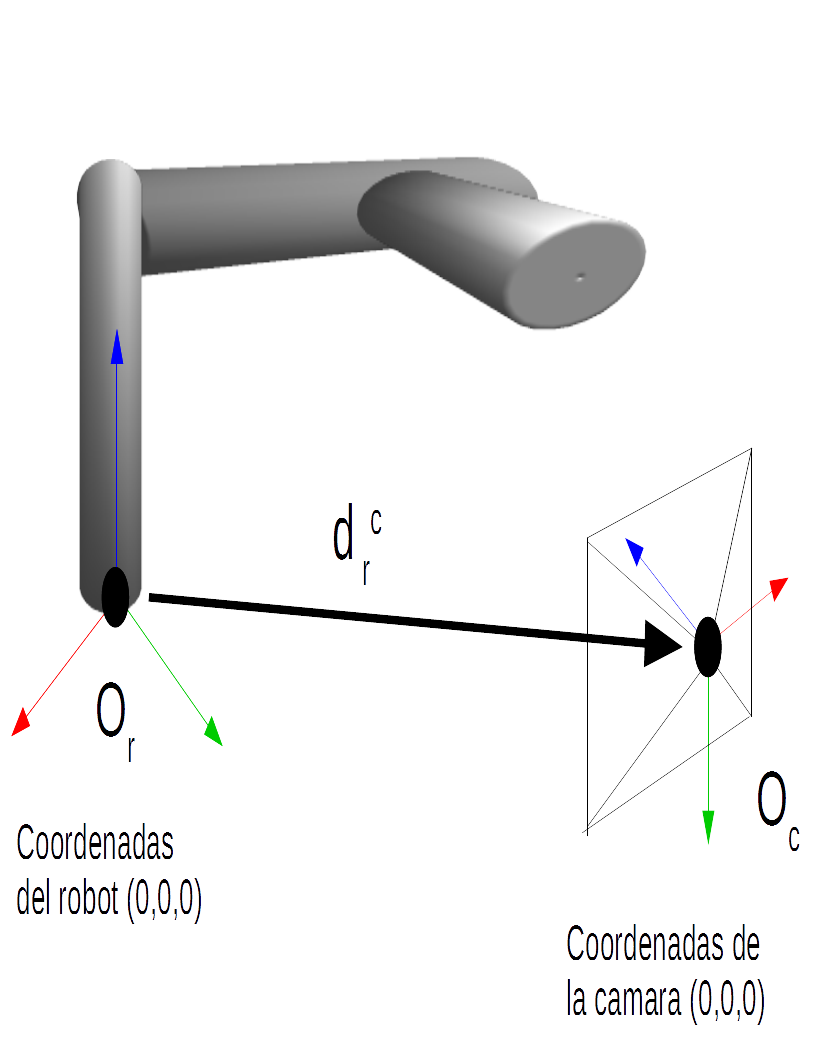
\includegraphics[width=0.5\linewidth]{visio/visio3/coordenadasrobcam2}
	\caption{Representacion de un Robot Cartesiano}
	\label{fig:coordenadasrobcam}
\end{figure}


\begin{figure}
	\centering
	\includegraphics[width=0.5\linewidth]{Imagenes/DSC_9825}
	\caption{}
	\label{fig:dsc9825}
\end{figure}



\subsection{\textit{Gripper}}
El \textit{Gripper} que vamos a utilizar es el modelo SCHUNK WSG-50 que aparece en \cref{fig:dsc9821}, tiene un observador de fuerza, utiliza una fuente de 24V, la abertura es de 10 cm y se puede utilizar con MATLAB para ser operado. \\
Para ser usado se necesitó establecer la comunicación con \textbf{MATLAB}, esta es comunicación básica, en la que se manda un paquete de datos que contiene el comando y las opciones, en el apéndice \ref{codewsg50}, aparece el código que se uso.

\begin{figure}
	\centering
	\includegraphics[width=0.7\linewidth]{Imagenes/DSC_9821}
	\caption{\textit{Gripper} modelo SCHUNK WSG-50}
	\label{fig:dsc9821}
\end{figure}

\subsubsection{base del \textit{Gripper}}
Se diseño la base para el \textit{Gripper}, y los dedos, se intenta usar el sensor de fuerza y momento, por lo que uno de los 2 dedos tiene una cavidad para este. en el apéndice \ref{label}, se puede encontrar el diseño que se uso.

en la imagen \ref{label}, se encuentra el resultado




\subsection{cámara}

El sistema de visión usa una cámara RGBD que se muestra en la figura \ref{fig:dsc9822}, se uso un programa entre MATLAB y Openni \cite{matlabwrapper}.

La cámara que se uso es el ASUS XTION PRO, su sensor de profundidad tiene un rango operativo de 0,8 metros a 3,5 metros, la resolución de la imagen de color y la imagen de profundidad es $480 \times640$, y la velocidad de fotogramas es 20 cuadros por segundo, ya que es la velocidad de fotogramas del sensor de profundidad. \\




\begin{figure}
	\centering
	\includegraphics[width=0.7\linewidth]{Imagenes/DSC_9823}
	\caption{Camara Asus Xtion live pro}
	\label{fig:dsc9823}
\end{figure}
\begin{figure}
	\centering
	\includegraphics[width=0.7\linewidth]{Imagenes/DSC_9824}
	\caption{}
	\label{fig:dsc9824}
\end{figure}


\section{Protocolo de Experimentación}

\section{Conclusiones}



    \chapter{Conclusiones Generales y Trabajo Final}











%\section{Conclusiones Generales}

De manera general en este trabajo se presento un método para remover objetos desconocidos de un área predeterminada, utilizando una imagen de profundidad y un sensor de fuerza y momentos.
El método propuesto tiene como finalidad lograr sujetar y remover un objeto que se encuentre dentro de un área predefinida, del cual no se tiene información previa.
Para la detección del objeto se discriminaron los puntos que estuvieran fuera del área de trabajo, y para la elección del punto de agarre se uso el centroide, el cual es calculado como la media de los puntos mas relevantes de las distancias del objeto. Dichos algoritmos, y tanto sus ventajas como desventajas se explican en el capitulo 2, y la importancia que tiene la calibración en este trabajo. 
En el capitulo 3 se presenta el modelo de control usado para el movimiento del robot cartesiano hacia la posición donde se encuentra el objeto, el cual consistía en un control neuro-difuso de nombre \textit{FREN}, el cual se presenta en \cite{fren}.
 
 En capitulo 4 se explicaron los conocimientos básicos del para la sujeción y el control que fue usado en el.
 
 
 Los resultados que fueron mostrados en el capitulo 5 demuestran que el método propuesto puede lograr la tarea deseada de forma aceptable%, y se observan las 
 
% los experimentosse realizaron.... 

%basandonos en las 

%\section{22222}

El mayor inconveniente de este acercamiento al problema de sujeción es que se necesitaría que fuese supervisado, lo cual va en contra de los objetivos deseados, como continuación se desea tener una base de datos que contenga los valores para una gran variedad de objetos.


Con respecto al hecho de conseguir el centroide con la cámara, esto no garantiza que corresponda con el centro de masas del objeto, la propuesta para este problema es calcularlo con el sensor de fuerza disponible, el cual es capaz de conseguir el \textit{Wrench}, teniendo 2 sensores de este tipo, en caso de que el centro de masas este en el centroide del objeto, ambos censores deberían tener mediciones iguales, pero en caso de que no sea este el caso los sensores deberían mostrar discrepancias en las mediciones y en base a estas debería poder calcularse el valor real del cetro de masas, lo que ayudaría conseguir información adicional acerca del objeto.
Por ultimo otro acercamiento al problema de la decisión de fuerza seria el hecho de tener una realimentación por parte de un sensor que mida el deslizamiento de la pieza, en este caso, es imposible de hacerse con la cámara, y los sensores de \textit{Wrench}, no son capaces de medirlo. En algunos trabajos ha sido reportado que el deslizamiento puede ser medido como un tipo de ruido por vibraciones debido a la rugosidad de las superficies rozándose, por lo que se podría tener también un indicador de la rugosidad entre el \textit{Gripper} y el objeto, por desgracia los sensores que se tienen, no son capaces de distinguir este ruido, esto sumado a que, en algunas áreas de la trayectoria, el mismo robot presenta una gran cantidad de vibraciones, para conseguir la medición de deslizamiento se pretende usar una matriz de resistencias que se tendrán en los dedos del \textit{Gripper}, esta matriz mostrara variaciones de voltaje dependiendo de la fuerza con la que se sujete la pieza, siempre y cuando exista el contacto entre ambos, con esto se puede crear una imagen de presión, de la cual se puede conseguir un centroide, este representaría el punto de contacto principal, en caso que existir un área de contacto. 

\section{Trabajo Futuro}

La siguiente sección fue presenta ideas para compensar algunas de las desventajas que se tienen en el sistema actual de visión, el cual, como ya se comento, no esta trabajando en linea.



La primer idea es identificar por medio de ambas cámaras, tanto a de color como la de profundidad, al objeto, y después conseguir con el Alg. \ref{alg2} el centroide y seguirlo con las características conseguidas con la cámara de color, sin seguir usando la cámara de profundidad, aplicando esto al objeto y al \textit{Gripper}, se esperaría tener un algoritmo propiamente de servo-visión.

Otro de los inconvenientes presentados es la necesidad de calibrar, o conocer los ángulos y las distancias que se tienen de la cámara al marco del robot, esto se pretende abordar teniendo el modelo 3D del \textit{Gripper}, una vez que se tenga este modelo se puede calcular las orientaciones entre el robot y la cámara, y con la medición de los sensores del robot, se tendría la posición actual del \textit{Gripper}, por lo que debería ser posible conseguir la distancia del robot a la cámara.







%%%%%%%%%%%%%%%%%%%%%%%%%%%%%%%%%%%%%%%%%%%%%%%%%%%%%%%%%%%%%%%%%%%%%%%%%%%%%%%%%%%%%%%%%%%%%%%%%%%%%
    \inputencoding{latin1}
    \appendix \part*{Ap\'endices}  \addcontentsline{toc}{part}{Ap\'endices}
    \inputencoding{utf8}
%%%%%%%%%%%%%%%%%%%%%%%%%%%%%%%%%%%%% Ap�ndices %%%%%%%%%%%%%%%%%%%%%%%%%%%%%%%%%%%%%%%%%%%%%%%%%%%
    \chapter{Cinemática del cuerpo rígido}
El cuerpo rígido es una forma básica de ver a los objetos en el espacio, estos objetos son parametrizados con 6 dimensiones con respecto a un marco de referencia, 3 de posición y 3 de orientación, al conjunto de estos valores se le conoce como \textbf{Pose}, el objeto tiene su propio marco de referencia al cual todos los puntos del objeto se mantienen constantes, pero se pueden mover con respecto del marco del origen, si el marco del objeto es rotado o trasladado, en \cref{fig:cuerporigido} se ilustra la idea general.

Análogamente se puede definir al \textbf{"Wrench"} como el conjunto de las fuerzas en y momentos que actúan sobre un cuerpo, pero se usa con otro propósito dentro de esta tesis.
A continuación se explicara de manera básica la manera de realizar una rotación y una traslación.

\begin{figure}[h]
	\centering
	\includegraphics[width=0.8\linewidth]{visio/visio3/cuerporigido}
	\caption{}
	\label{fig:cuerporigido}
\end{figure}

\section{Matriz de rotación}

En álgebra lineal las matrices de rotación se usan para realizar una rotación en un espacio euclidiano.

Las rotaciones básicas son las que se llevan acabo en un solo eje, las siguientes son las rotaciones básicas:

$R_x(\theta)=\begin{bmatrix}
1	& 0 &0  \\ 
0	&  cos(\theta)& -sin(\theta) \\ 
0	& sin(\theta) & cos(\theta) 
\end{bmatrix}\\

R_y(\theta)=\begin{bmatrix}
	cos(\theta)	& 0 & sin(\theta)  \\ 
	0	&  1 & 0 \\ 
	-sin(\theta)	& 0 & cos(\theta) 
\end{bmatrix}\\

R_z(\theta)=\begin{bmatrix}
	cos(\theta)	& -sin(\theta) &0  \\ 
	sin(\theta)	&  cos(\theta)& 0 \\ 
	0	&  & 1 
\end{bmatrix}\\
$
Desde estas rotaciones se define la rotación general como $R_{xyz}(\psi,\theta,\phi)=R_x(\psi)R_y(\theta)R_z(\phi)$, esto se puede pensar como una serie de rotaciones
\begin{equation}\label{rotation}
{\small R_{xyz}(\theta)=\begin{bmatrix}
cos(\psi)cos(\theta)cos(\phi)-sin(\psi)sin(\phi)	& -cos(\psi)cos(\theta)sin(\phi) -sin(\psi)cos(\phi) & cos(\psi)sin(\theta)   \\ 
sin(\psi)cos(\theta)cos(\phi)+cos(\psi)sin(\phi) &  -sin(\psi)cos(\theta)sin(\phi) +cos(\psi)cos(\phi) &  sin(\psi)sin(\theta) \\ 
sin(\theta)cos(\phi)	& sin(\theta)sin(\phi) & cos(\theta) 
\end{bmatrix}\\}
\end{equation}


para realizar una rotación se realiza la siguiente operación.


c'=Rc



por ejemplo una rotación básica en el eje x

$\begin{bmatrix}
	x  \\ 
	y' \\ 
	z'
\end{bmatrix} =\begin{bmatrix}
1	& 0 &0  \\ 
0	&  cos(\theta)& -sin(\theta) \\ 
0	& sin(\theta) & cos(\theta) 
\end{bmatrix} \begin{bmatrix}
	x  \\ 
	y \\ 
	z
\end{bmatrix} $, como se puede apreciar, no se afecta x al ser el eje de rotación.


En la sección de visión se utilizo la matriz de rotación general \ref{rotation} parametrizada en ángulos de Euler.

\section{traslación}

Una traslación se usa en el algoritmo de visión para posicionar el origen de las coordenadas de la imagen junto al origen de las coordenadas del robot, para hacer esto se lleva a cavo una resta.
esta operación se define como:  las nuevas coordenadas de la imagen son las coordenadas desde la cámara menos la distancia entre el origen de la cámara con respecto al origen del robot.
$p_{nuevo}=p_c-d_{r}^{c}$

por ejemplo:

$\begin{bmatrix}
x'  \\ 
y' \\ 
z'
\end{bmatrix} = 
\begin{bmatrix}
x  \\ 
y \\ 
z
\end{bmatrix}-\begin{bmatrix}
d_x	 \\ 
d_y	 \\ 
d_z	 
\end{bmatrix} $





\chapter{Bases de Redes Neuro-Difusas}\label{basesneurodifusas}
En la inteligencia artificial existen varios tipos de control, estos son biomimeticos, ya que están basados en la naturaleza, en este capitulo se hablara acerca de la lógica difusa y las redes neuronales para facilitar el entendimiento de las ANFIS(Sistemas Adaptativos de Inferencia Neuro-Difusa).

\section{Lógica Difusa}

La lógica difusa es una rama de la inteligencia artificial que usa una lógica booleana modificada para que puedan usarse estados medios entre las variables haciendo mas suave su respuesta, normalmente se usa de forma orientada a la aplicación, ya que se usa conocimiento especifico de la planta para el diseño del control, aunque en muchos casos se puede simplificar a minimizar el error. 
Básicamente el control difuso convierte datos numéricos a valores difusos, estos son evaluados por un mecanismo de inferencia quien decide la respuesta del controlador basado en las reglas difusas, por ultimo se traducen los resultados a valores apropiados para la planta, la estructura básica de un control difuso se muestra en \cref{fig:logicadifusa}.

\begin{figure}[h]
	\centering
	\includegraphics[width=1\linewidth]{visio/visio3/logicadifusa}
	\caption{}
	\label{fig:logicadifusa}
\end{figure}

El control difuso se basa en las reglas difusas, estas son un conjunto de reglas Si... Entonces... , y están basadas en la experiencia humana acerca de la planta, comúnmente en forma de tabla con entradas y salidas, se pueden tener múltiples entradas, pero se sugiere tener solo una salida, y para conseguir mas salidas se usan varios controles de una entrada. Un ejemplo de estas reglas es, en el caso que se tenga una relación directa y proporcional de la entrada de control con la salida del sistema: "Si el \textbf{error} es positivo y el \textbf{error anterior} es positivo, entonces la \textbf{respuesta} es/sera negativa", como puede verse de este ejemplo, las reglas en si son básicamente lo que una persona entiende del comportamiento del sistema, y deben contemplar todas las situaciones posibles, en caso de no hacerlo, puede llegar a caerse en situaciones desconocidas en las que el control no sabrá como reaccionar y puede llevar a reacciones no deseadas por parte del control. Algo mas que debe observarse es la relación que tienen las variables que se asemeja a la lógica booleana, pero la lógica difusa se distingue de la booleana por el tipo de variables que usa, mientras la lógica booleana usa valores discretos que solo pueden ser cierto o falso, la lógica difusa intenta aprovechar los números que estén en medio, agregando un grado de certeza a cada variable, por lo que una variable difusa puede tomar valores de 0 hasta 1, esto permite tener mas posibles valores en las variables sin necesidad de aumentar su numero.
La conversión de la entrada a datos difusos es comúnmente llamada  fusificación, las entradas son generalmente valores numéricos, la manera de realizar la fusificación es definir cuales son las variables de entrada y los valores lingüísticos que cada una se puede tomar, en el ejemplo se puede identificar que la entrada esta siendo comparada contra algo en la frase "Si el error es positivo", el \textbf{error} es la variable, y \textbf{positivo} es un valor lingüístico, dependiendo de los valores que puedan tomar las variables de entrada serán los valores lingüísticos que se tengan, en este caso la variable podría tomar los valores de \textbf{positivo} y \textbf{negativo}, también se puede agregar \textbf{cero}, pero lo mas común es que los valores numéricos de la entrada sean convertidos a valores lingüísticos que describan su intensidad, por ejemplo si se quisiera describir mejor a \textbf{error}, lo mas común es usar: \textbf{positivo grande},  \textbf{positivo pequeño}, \textbf{cero}, \textbf{negativo pequeño} y \textbf{negativo grande}. 
Ahora que ya están definidos se elige una función que describa que tan cierta es cada situación, estas son llamadas funciones de membresía y valúan cada entrada con cada una de las funciones, que representan los valores lingüísticos dependiendo de las reglas difusas, para esto se usan funciones triangulares que son simples y rápidas o funciones gausianas que tienen un cambio suave, cuando las entradas son valuadas con estas funciones, se conseguirán valores de 0 a 1, y por lo general se activaran mas de un valor lingüístico, en caso de que solo se active 1 valor lingüístico se recomienda que su valor sea siempre de 1, en caso de caer este valor, el control perderá fuerza, por lo que se sugiere tener el valor normalizado, por ejemplo si decimos que el error es \textbf{positivo grande}, dependiendo de la magnitud del error este podría estar solo en la región de \textbf{positivo grande} al 100\%, pero en caso de ser mas pequeño, podría entrar en una parte donde \textbf{positivo grande} se activa al 60\% y \textbf{positivo pequeño} se activa al 40\%.

El mecanismo de inferencia hace uso de las reglas difusas evaluándolas todas con las funciones de membresía, con esto se observa que tan cierta es cada una de las reglas y que tan cierto debería ser cada respuesta, dependiendo del método de des-fusificación que se use se conseguirá la respuesta.

Ahora cambiando un poco la regla de ejemplo: "Si el \textbf{error} es positivo grande y el \textbf{error anterior} es positivo pequeño, entonces la \textbf{respuesta} es/sera negativa grande", como ya se había dicho la lógica difusa es una modificación de la lógica de bool, por lo tanto los operadores lógicos "$y$", "$o$", son usados, pero de forma mas sencilla para una persona. Estos operadores lógicos pueden ser, sumas y multiplicaciones, o el máximo y el mínimo, siguiendo con el ejemplo, reemplazando los valores, imaginemos que las funciones de membresía, solo para esta regla son $\mu_{error}=0.6$ y $\mu_{errorant}=0.4$, cuando se aplica el operador lógico \textbf{y}, se tendrá 0.4 en caso de usar el mínimo o 0.24 en caso de un producto, este valor es el grado de "certeza" que se tiene de esta regla, y la respuesta de la regla "entonces la \textbf{respuesta} es/sera negativa grande", también es afectada por este valor, la respuesta del mecanismo de inferencia es el conjunto de las  respuestas de todas las reglas.
Finalmente para poder usar esta respuesta se le debe dar un valor numérico, esto es llamado des-fusificación y se pueden usar métodos como la media del centro de cada respuesta, o en el caso de los sistemas Takagi-Sugeno, se puede calcular una respuesta numérica para cada regla y sumarlas para conseguir la respuesta final.


\section{Redes Neuronales}
Las redes neuronales son una rama de la inteligencia artificial que imita el comportamiento de las neuronas, una de las características mas importantes es que no se necesita tener conocimiento especifico de la planta, ya que la red aprenderá en base al entrenamiento que se le de. La forma básica de una neurona es la mostrada en \cref{fig:neurona}, como puede verse tiene 3 partes, principales, ya que las entradas son solo asignaciones, en la sección de pesos lo que se hace es multiplicar cada una de las entradas por su respectivo peso, después se suman todos los resultados y al final se pasa a una función de activación que decidirá el resultado final. 
\begin{figure}[h]
	\centering
	\includegraphics[width=.9\linewidth]{visio/visio3/neurona}
	\caption{}
	\label{fig:neurona}
\end{figure}
La función de salida se puede condensar como y=G(z), donde $ z=\sum(in_1 W_1 + in_2 W_2 + in_3 W_3)$, note que esta operación puede ser simplificada como el producto punto del vector de entradas y el vector de pesos, y en cuanto a la función G(), esta es elegida por el usuario, la mas comun es una linea o una sigmoide, pero pueden usarse otras como una gausiana. Los valores de los pesos son inicializados en ceros y van cambiando conforme se tenga entrenamiento.



\chapter{Diseño}
Se presenta el diseño de uno de los dedos del \textit{gripper}.

\begin{figure}[h]
	\centering
	\includegraphics[width=1\linewidth]{visio/visio3/finger4}
	\caption{}
	\label{fig:finger4}
\end{figure}

%014772670930 3570 guadalupe martinez
\chapter{Publicaciones}
\cite{tuyinincluded2017}

    \definecolor{gray97}{gray}{.97}
\definecolor{bluekeywords}{rgb}{0.13,0.13,1}
\definecolor{greencomments}{rgb}{0,0.5,0}
\definecolor{redstrings}{rgb}{0.9,0,0}
%\DeclareCaptionFormat{listing}{\colorbox{gray}{\parbox{\textwidth}{#1#2#3}}}
%\captionsetup[lstlisting]{format=listing,labelfont=white,textfont=white}

\lstset{language=Matlab, %c#  ó c++
showspaces=false,
showtabs=false,
breaklines=true,
showstringspaces=false,
breakatwhitespace=true,
escapeinside={(*@}{@*)},
keywordstyle=\color{bluekeywords}\bfseries,
backgroundcolor=\color{gray97},
%%%
numberstyle=\footnotesize,
numbers=left,
stepnumber=1,
numbersep=10pt,
tabsize=2,
breaklines=true,
prebreak = \raisebox{0ex}[0ex][0ex]{\ensuremath{\hookleftarrow}},
breakatwhitespace=false,
aboveskip={1.5\baselineskip},
columns=fixed,
upquote=true,
extendedchars=true,
frame=lines,
}
\chapter{Código de programación}\label{codigo}

Ejemplo de un código de programación:

\section{Anexo I. Código de visión}\label{visioncode}
 \begin{lstlisting}
 D=permute(D,[2 1 3]);
 tic
 coor(:,1)=reshape(D(:,:,1),[sx*sy,1]);
 coor(:,2)=reshape(D(:,:,2),[sx*sy,1]);
 coor(:,3)=reshape(D(:,:,3),[sx*sy,1]);
 newcoor=coor*R;
 x=reshape(newcoor(:,1),[sy,sx])+dx;
 y=reshape(newcoor(:,2),[sy,sx])+dy;
 z=reshape(newcoor(:,3),[sy,sx])+dz;
 
 y(x>maxX)=nan;
 z(x>maxX)=nan;
 x(x>maxX)=nan;
 
 x(or(y<maxY,y>minY))=nan;
 z(or(y<maxY,y>minY))=nan;
 y(or(y<maxY,y>minY))=nan;
 
 x(z>maxZ)=nan;
 y(z>maxZ)=nan;
 z(z>maxZ)=nan;
 
 xyz=cat(3,x,y,z);
 %figure;mesh(xyz(:,:,1),xyz(:,:,3),xyz(:,:,2))
 %axis equal
 
 
 
 mx=mean(x(dix~=0));
 my=mean(y(diy~=0));
 mz=mean(z(diz~=0));
 %despues se consigue el error con respecto de x
 erx=abs(x-mx);
 raycasting=z((erx<5));
 %pz(l)=max(raycasting);
 %py(l)=my;
 %px(l)=mx;
 %raycastedy=y((erx<5));
 %wi(l)=max(raycastedy)-min(raycastedy);
 
 t(l)=toc;
 end
 
 dpos=[px py pz];
 \end{lstlisting}

\section{Anexo II. Código de FREN}\label{FRENcode}

\subsection{Evaluación de FREN}
\begin{lstlisting}
function [lc, per]=fren(member,ship)
type=ship.type;
class=ship.class;
c=ship.c;
b=ship.b;
betas=ship.betas;
f=ship.f;
%per=zeros(1,l);
switch class
case 'fren'
l=ship.l;

switch type
case 'tri'
pass=ship.pass;
for i=1:l
for j=1:3
if pass{i}{j}(member,c(i),b(i))
per(i)=f{i}{j}(member);
end
end
end
case 'gauss'
for i=1:l
per(i)=f{i}{1}(member,c(i),b(i));
end

end
lc=per*betas';

case 'frend'
index=ship.index;
switch type

case 'gauss'
for j=1:index
for i=1:length(c{j})
per{j}(i)=f{j}{i}{1}(member(j),c{j}(i),b{j}(i));
end 
per{j}=per{j}./sum(per{j});
end


if mod(index,2)==1
ain=index;
bin=index-1;
else
ain=index-1;
bin=index;
end
[a,~]=rekron(per,ain,'evaluation');
[b,~]=rekron(per,bin,'evaluation');
%   lc=per*betas'*perd*betasd';  %check
lc=a*betas*b';
end
end

end
\end{lstlisting}


\subsection{Creación de una FREN}
\begin{lstlisting}
function ship=shipconstruction(class,type,center,base,betas,y,eta)

switch class

case 'fren'
l=length(center);
ship=struct('class',class,'type',type,'c',center,'b',base,'l',l,'betas',betas,'y',y,'eta',eta);

syms mem
switch type
case 'tri'
passi={@(mem,c,b)(mem<=c),@(mem,c,b)(mem>=c)&&(mem<=(c+b)),@(mem,c,b)(mem>=(c+b))};
passm={@(mem,c,b)(mem<=c)&&(mem>=c-b),@(mem,c,b)(mem>=c)&&(mem<=c+b),@(mem,c,b)(mem<=c-b)||(mem>=c+b)};
passf={@(mem,c,b)(mem>=c),@(mem,c,b)(mem<=c)&&(mem>=c-b),@(mem,c,b)(mem<=c-b)};

ship.pass{1}=passi;
f=(-1/base(1))*mem+(center(1)/(base(1))+1);
f=cat(2,'@(mem)',char(f));
a=str2func(f);
ship.f{1}={@(mem)1,a,@(mem)0};
for i=2:l-1
ship.pass{i}=passm;
f=(1/base(i))*(mem-center(i))+1;
f=cat(2,'@(mem)',char(f));
a=str2func(f);
f=(-1/base(i))*mem+(center(i)/(base(i))+1);
f=cat(2,'@(mem)',char(f));
b=str2func(f);
ship.f{i}={a,b,@(mem)0};
end
ship.pass{l}=passf;
f=(1/base(1))*mem+(center(1)/(base(1))+1);
f=cat(2,'@(mem)',char(f));
a=str2func(f);
ship.f{l}={@(mem)1,a,@(mem)0};

case '+-'

case 'gauss'
syms In a b
Mu=(1./(1+exp(2*pi*(1/b)*(In-a-b/2))));
f=cat(2,'@(In,a,b)',char(Mu));
f=str2func(f);
ship.f{1}={f};
for i=2:l-1
f=exp(-((In-a)^2)/(b^2/pi));
f=cat(2,'@(In,a,b)',char(f));
f=str2func(f);
ship.f{i}={f};
end
Mu=(1./(1+exp(-2*pi*(1/b)*(In-a+b/2))));
f=cat(2,'@(In,a,b)',char(Mu));
f=str2func(f);
ship.f{l}={f};

case 'tan'

end

=========================== MiFREN=============================
case 'frend'
index=length(center);
ship=struct('class',class,'type',type,'index',index,'y',y,'eta',eta);
ship.c=center;
ship.b=base;
%        ship.betas=betas;
[ship.betas,~]=rekron(betas,index,'construction');
switch type
case 'gauss'

syms In a b
for j=1:index
l=length(center{j});
Mu=(1./(1+exp(2*pi*(1/b)*(In-a-b/2))));
f=cat(2,'@(In,a,b)',char(Mu));
f=str2func(f);
ship.f{j}{1}={f};
for i=2:length(center{j})-1
f=exp(-((In-a)^2)/(b^2/pi));
f=cat(2,'@(In,a,b)',char(f));
f=str2func(f);
ship.f{j}{i}={f};
end
Mu=(1./(1+exp(-2*pi*(1/b)*(In-a+b/2))));
f=cat(2,'@(In,a,b)',char(Mu));
f=str2func(f);
ship.f{j}{l}={f};
end
end
end
\end{lstlisting}

\subsection{fase de aprendizaje}
\begin{lstlisting}
function ship=shipmodernization(ship,per,e)
y=ship.y;
betas=ship.betas;
eta=ship.eta;

class=ship.class;
switch class
case 'fren'
ship.betas=betas+eta*y*e*per;
case 'frend'
ship.betas=betas+eta*y*e*per;
end
\end{lstlisting}

\subsection{Programa de recursivo para producto \textbf{Kroneker}}
\begin{lstlisting}
function [w,index]=rekron(crew,index,type)
a=crew{index};

switch type
case 'construction'
if index==2
w=kron(a,crew{1}');
elseif mod(index,2)==1
w=kron(a,rekron(crew,index-1,'construction')')';
elseif mod(index,2)==0
w=kron(a,rekron(crew,index-1,'construction'));
end

case 'evaluation'
if index<=2
w=a;
elseif index>2
w=kron(a,rekron(crew,index-2,'evaluation'));
end

end
\end{lstlisting}


\section{Anexo III. Comunicación con WSG50}\label{codewsg50}
\begin{lstlisting}
%comunication
%obj = tcpip('192.168.1.20', 1000, 'NetworkRole', 'client');
%fopen(obj)
function [id, statuscode, payload] =wsg50(obj,cmd,stat)
%==============//////////note: falta check sum////////==================
%command
%check database, this migth take some time
% id='a';
% statuscode='b'; 
% payload='c';
if nargin ==3
stat=single(stat);
end
switch cmd

case 'connect'
%   obj = tcpip('192.168.1.20', 1000, 'NetworkRole', 'client');
obj.ByteOrder = 'littleEndian';
fopen(obj);
return

case 'disconnect'
%   cmd='07';
pack={ 'AA', 'AA', 'AA', '07', '00', '00',  '35', '4C'};
fwrite(obj,hex2dec(pack),'char')
fclose(obj);
id=0;
return
case 'homing'
%   cmd='20';
pack={ 'AA', 'AA', 'AA', '20', '01', '00', dec2hex(stat), '00', '00'};

case 'preposition'
%   cmd='21';
v=num2hex([stat(2),stat(3)]);
pack={ 'AA', 'AA', 'AA', '21', '09', '00', dec2hex(stat(1)),v(1,7:8),v(1,5:6),v(1,3:4),v(1,1:2),v(2,7:8),v(2,5:6),v(2,3:4),v(2,1:2), '00', '00'};

case 'stop'
%   cmd='22';
pack={ 'AA', 'AA', 'AA', '22', '00', '00', '00', '00'};

case 'faststop'
%   cmd='23';
pack={ 'AA', 'AA', 'AA', '23', '00', '00', '00', '00'};

case 'aknwfaststop'
%   cmd='24';
pack={ 'AA', 'AA', 'AA', '24', '03', '00', '61', '63', '6B' , '00', '00'};

case 'grip'
%   cmd='25';
v=num2hex([stat(1),stat(2)]);
pack={ 'AA', 'AA', 'AA', '25', '08', '00',v(1,7:8),v(1,5:6),v(1,3:4),v(1,1:2),v(2,7:8),v(2,5:6),v(2,3:4),v(2,1:2), '00', '00'};

case 'release'
%   cmd='26';
v=num2hex([stat(1),stat(2)]);
pack={ 'AA', 'AA', 'AA', '26', '08', '00',v(1,7:8),v(1,5:6),v(1,3:4),v(1,1:2),v(2,7:8),v(2,5:6),v(2,3:4),v(2,1:2), '00', '00'};

case 'dforce'
%   cmd='32';
v=num2hex(stat);
pack={ 'AA', 'AA', 'AA', '32', '04', '00',v(1,7:8),v(1,5:6),v(1,3:4),v(1,1:2), '00', '00'};

case 'opening?'
%   cmd='43';
v=dec2hex(cat(2,stat,4096));
pack={ 'AA', 'AA', 'AA', '43', '03', '00',v(1,3:4),v(2,3:4),v(2,1:2), '00', '00'};

case 'speed?'
%   cmd='44';
v=dec2hex(cat(2,stat,4096));
pack={ 'AA', 'AA', 'AA', '44', '03', '00',v(1,3:4),v(2,3:4),v(2,1:2), '00', '00'};

case 'force?'
%   cmd='45';
v=dec2hex(cat(2,stat,4096));
pack={ 'AA', 'AA', 'AA', '45', '03', '00',v(1,3:4),v(2,3:4),v(2,1:2), '00', '00'};

case 'read'
[id, statuscode, payload] = read_data(obj);
return

otherwise
disp('command not implemented')
return
end

fwrite(obj,hex2dec(pack),'char')
% estaparte deberia ser usada aparte, despues del  comando, o como cotro
% comando
% disp('1');
[id, statuscode, payload] = read_data(obj); %wait for acknowledgement
% disp('2');
%  [id(:,:,2), statuscode(:,:,2), payload(:,:,2)] = read_data(obj); %wait for command to be executed


function [command_id, statuscode, payload] = read_data(t)
%wait for preamble
command_id=nan;
statuscode=nan;
payload=nan;

while (fread (t,1) ~= 170)  
end;
fread (t,2);  %read the rest of the preamble
%read the command ID
command_id = fread (t,1);
%read the length of the payload (two bytes)
length= fread (t,1,'uint16');
%read the status code (two bytes)
statuscode = fread(t, 1, 'uint16');

switch statuscode
case 0
statuscode='success';
case 1
statuscode='data not avaible';
case 2
statuscode='no sensor';
case 3
statuscode='not initialized';
case 4
statuscode='already running';
case 5
statuscode='not suported';
case 6
statuscode='inconsistent data';
case 7
statuscode='timeout';
case 8
statuscode='read error';
case 9
statuscode='write error';
case 10
statuscode='low memory';
case 11
statuscode='checksum';
case 12
statuscode='no parameter expected';
case 13
statuscode='not enough parameters';
case 14
statuscode='unkwn cmd';
case 15
statuscode='format error';
case 16
statuscode='access denied';
case 17
statuscode='already open';
case 18
statuscode='error while excecuting the comand';
case 19
statuscode='cmd aborted';
case 20
statuscode='invalid ahndle';
case 21
statuscode='device or file not found';
case 22
statuscode='device or file not open';
case 23
statuscode='i/o error';
case 24
statuscode='wrong parameter';
case 25
statuscode='index out of bounds';
case 26
statuscode='cmd pending';
case 27
statuscode='data overrun';
case 28
statuscode='range error';
case 29
statuscode='axis blocked';
case 30
statuscode='file already exist';
end


if strcmp(statuscode,'success')
length = length - 2;
else
length=0;
return
end

%decrease the length of the payload by the statuscode bytes

%read the payload
if ( length > 0 )
payload = fread(t, length);
payload = double(typecast(uint8(payload), 'single'));
else
payload = 0 ;
end
%read the checksum
% checksum = fread (t, 1,'uint16');
\end{lstlisting}


\section{Anexo IV. Código Completo}\label{codefull}
\begin{lstlisting}
% robot 1.8
%------change log--------------------------------------------------------------
% 1.6   este tiene la funcion freen.m
% 1.7   aqui se agrega la parte 2.5D  
% 1.8   este es cuando se hace en lazo abierto.
%---------------------------------------------------------------------
for l=1:1
clear;
%% -------  CONTROL --------
center=[-5 -2 0 2 5];
base=[3 2 2 2 3];
betas=[-5000 -500 1e-6 500 5000];
% shipx=shipconstruction('fren','gauss',center,base,betas,1,1);
shipx=shipconstruction('gauss',center,base,betas,1,1);

shipy=shipx;
shipz=shipx;

%% vision
%%%antes
load gripperfeatures.mat
close all;
addpath('Mex')
SAMPLE_XML_PATH='Config/SamplesConfig.xml';
KinectHandles=mxNiCreateContext(SAMPLE_XML_PATH);
%%% variables
iter=5;
tolerance=.3;
inicial=41;
final=440;
totaly=final-inicial;
gripperarea=4700; %esto tal vez no sea necesario
trigger=0;
target='lost';
delta=.3;
flagj=0;
flagi=0;
minZ=700;
maxZ=1000;
object=struct('cent',[0,0],'area',0,'box',[0 0 0 0],'x',0,'y',0);
gripper=struct('cent',[0,0],'area',0,'box',[0 0 0 0],'x',0,'y',0);
se90 = strel('line', 5, 90);
se0 = strel('line',5, 0);


%% INIT-INSTRUMENTS
obj2 = instrfind('Type', 'visa-gpib', 'RsrcName', 'GPIB0::10::0::INSTR', 'Tag', '');

% Create the VISA-GPIB object if it does not exist
% otherwise use the object that was found.
if isempty(obj2)
obj2 = visa('NI', 'GPIB0::10::0::INSTR');
else
fclose(obj2);
obj2 = obj2(1)
end

% Connect to instrument object, obj2
set (obj2,'OutputBufferSize',100000);
fopen(obj2);

fprintf (obj2, '*IDN?');
idn = fscanf (obj2);
fprintf (idn)
fprintf ('\n\n')

%Clear and reset instrument
fprintf (obj2, '*RST');
fprintf (obj2, '*CLS');

%Set desired configuration.
fprintf(obj2,'FUNCTION SQU');
fprintf(obj2,'VOLT 2.5'); % set max waveform amplitude to 2 Vpp
fprintf(obj2,'VOLT:OFFSET 1.25'); % set offset to 0 V
fprintf(obj2,'OUTPUT:LOAD 50'); % set output load to 50 ohms


% System input/output definiftion--------------

do=digitalio('nidaq','Dev1');     % Data to move motors 
addline(do,0:5,'Out');

DIRX=1;
DIRY=2;
DIRZ=3;


MX=4;
MY=5;
MZ=6;

RIGHT=1;
LEFT=0;

ON=1; 
OFF=0;

% Add initial for function GEN 
putvalue(do.line(MX),ON);
putvalue(do.line(MY),ON);
putvalue(do.line(MZ),OFF);
% -------------  

%% ---------Constants for position----------
kmax=1000;
u_max=20000;
u=zeros(1,kmax+1);

xd=u;%preallocation, en caso de que se quiera seguir una trayectoria, si se quiere constante, borrar xd"(k+1)"
x=u;
y=u;
z=u;
e=zeros(kmax+1,3);
eo=e;
Ts=u;
R_Time=u;
km=6.0049;
kb=-0.054;

%---Voltage reading 
aiv=analoginput('nidaq','Dev1')
addchannel(aiv,0)
set(aiv,'InputType','SingleEnded')
V_z=getsample(aiv);    % Read the voltage ... 
PosZ=km*V_z+kb;
x(1)=PosZ(1);  % Psition  [cm]






%% Control Force Loop

% ------ Turn ON Function Gen -----
fprintf(obj2,'OUTPUT ON');
F_END=0;
fprintf(obj2,['FREQ ', num2str(F_END)]); %set frequency to Hz
end

% while resp==r
% i=1;
% ra=10;
% s.BaudRate=ra*i;
% fopen(s);
% resp=fscanf(s)
% fclose(s);
% if i>1000
%     break
% end
% end

%------------------ parte 2.5D ------------------

mxNiUpdateContext(KinectHandles);
D=mxNiDepthRealWorld(KinectHandles);

sx=640;
sy=480;

maxX=1600;
maxY=-1600;
maxZ=1450;
minY=1000;
dx=-500;
dy=1000;
dz=200;


al=(0)*pi/180;
be=(0)*pi/180;
ga=(0)*pi/180;

rx=[1 0 0;0 cos(al) -sin(al);0 sin(al) cos(al)];
ry=[cos(be) 0 sin(be);0 1 0;-sin(be) 0 cos(be)];
rz=[cos(ga) -sin(ga) 0;sin(ga) cos(ga) 0;0 0 1];
R=rx*ry*rz;

for l=1:1

D=permute(D,[2 1 3]);
tic
coor(:,1)=reshape(D(:,:,1),[sx*sy,1]);
coor(:,2)=reshape(D(:,:,2),[sx*sy,1]);
coor(:,3)=reshape(D(:,:,3),[sx*sy,1]);
newcoor=coor*R;
x=reshape(newcoor(:,1),[sy,sx])+dx;
y=reshape(newcoor(:,2),[sy,sx])+dy;
z=reshape(newcoor(:,3),[sy,sx])+dz;

y(x>maxX)=nan;
z(x>maxX)=nan;
x(x>maxX)=nan;

x(or(y<maxY,y>minY))=nan;
z(or(y<maxY,y>minY))=nan;
y(or(y<maxY,y>minY))=nan;

x(z>maxZ)=nan;
y(z>maxZ)=nan;
z(z>maxZ)=nan;

xyz=cat(3,x,y,z);
%figure;mesh(xyz(:,:,1),xyz(:,:,3),xyz(:,:,2))
%axis equal



mx=mean(x(dix~=0));
my=mean(y(diy~=0));
mz=mean(z(diz~=0));
%despues se consigue el error con respecto de x
erx=abs(x-mx);
raycasting=z((erx<5));
%pz(l)=max(raycasting);
%py(l)=my;
%px(l)=mx;
%raycastedy=y((erx<5));
%wi(l)=max(raycastedy)-min(raycastedy);

t(l)=toc;
end

dpos=[px py pz];
%------------------- Main Loop ----------------
R_Time(1)=0;
for k=1:kmax-1 
%% position
V_x=getsample(aiv);    % Read the voltage ...
pos=km*V_x+kb;


%% freen control
eu=dpos-pos; %e(iter,:)%mean(e(k-2:k,:))
if  abs(eu(1))>10
putvalue(do.line(MX),ON);
putvalue(do.line(MY),OFF);
putvalue(do.line(MZ),OFF);
[u_tempx, perx]=fren(eu(1),shipx);
% display(eu(1));
display(u_tempx);

if abs(u_tempx)>u_max
u(k)=sign(u_tempx)*u_max;
else
u(k)=u_tempx;
end1

%--- Send control effort to system ---
if u(k)>=0
putvalue(do.line(DIRX),RIGHT);  % Down --
else
putvalue(do.line(DIRX),LEFT);  % Up --
end
F=abs(u(k));
fprintf(obj2,['FREQ ', num2str(F)]); %set frequency to Hz
%--------------------------------------

shipx=shipmodernization(shipx,perx,eu(1));
end
end




if 0%abs(eu(3))>10
putvalue(do.line(MX),OFF);
putvalue(do.line(MY),ON);
putvalue(do.line(MZ),OFF);
[u_tempy, pery]=fren(eu(3),shipy);
% display(eu(3));
display(u_tempy);

if abs(u_tempy)>u_max
u(k)=sign(u_tempy)*u_max;
else
u(k)=u_tempy;
end
%--- Send control effort to system ---
if u(k)>=0
putvalue(do.line(DIRY),0);  % Down --
else
putvalue(do.line(DIRY),1);  % Up --
end
F=abs(u(k));
fprintf(obj2,['FREQ ', num2str(F)]); %set frequency to Hz
%--------------------------------------

shipy=shipmodernization(shipy,pery,eu(3));
end


if 0%abs(eu(2))>10
putvalue(do.line(MX),OFF);
putvalue(do.line(MY),OFF);
putvalue(do.line(MZ),ON);
[u_tempz, perz]=fren(eu(2),shipx);
% display(eu(2));
display(u_tempz);

if abs(u_tempz)>u_max
u(k)=sign(u_tempz)*u_max;
else
u(k)=u_tempz;
end


%--- Send control effort to system ---
if u(k)>=0
putvalue(do.line(DIRZ),RIGHT);  % Down --
else
putvalue(do.line(DIRZ),LEFT);  % Up --
end
F=abs(u(k));
fprintf(obj2,['FREQ ', num2str(F)]); %set frequency to Hz
%--------------------------------------
shipz=shipmodernization(shipz,perz,eu(2));
end
Ts(k) = toc(tstart);
R_Time(k+1)=R_Time(k)+Ts(k);


if sum(abs(eu))==0
putvalue(do.line(MX),OFF);
putvalue(do.line(MY),OFF);
putvalue(do.line(MZ),OFF);
end
toc
tic
end



%% fin

for l=1:1
delete (aiv);

F_END=0;
fprintf(obj2,['FREQ ', num2str(F_END)]); %set frequency to Hz

%------Turn OFF All Instruments and motor --------

putvalue(do.line(MX),OFF);
putvalue(do.line(MY),OFF);
putvalue(do.line(MZ),OFF);
delete(do);

fprintf(obj2,'OUTPUT OFF');
fclose(obj2);
% 
% y_final=xd(k+1);
mxNiDeleteContext(KinectHandles)
end
\end{lstlisting} % Si no se requiere %
    \backmatter          %%----------------------------
    \inputencoding{latin1}
    \bibliographystyle{Archivos/apalike} \addcontentsline{toc}{part}{Bibliograf\'ia}
    %\nocite{*}
    \bibliography{Archivos/Bibliografia} % Bibliografia con ejemplos, para modificar doble click en \bibliography
\end{document}
